\documentclass[8pt, xcolor={svgnames}, hyperref={linkcolor=black}]{beamer}
\usepackage[labelfont={color=amethyst,bf}]{caption}
\setbeamercolor{background canvas}{bg=white}
\usetheme[progressbar=frametitle]{metropolis}
\usepackage{appendixnumberbeamer}
\usepackage{url}
\usepackage{booktabs}
\usepackage{braket}
\usepackage[scale=2]{ccicons}
\usepackage{amsfonts} 
\usepackage{amssymb}
\usepackage[english]{babel}
\colorlet{col1}{teal}
\colorlet{col2}{yellow}
\colorlet{col3}{green}
\usepackage{fontawesome}
\usepackage{subcaption}
\usepackage{multicol}
\usepackage{bm}
\usepackage{algorithm}
\usepackage{algpseudocode}
\usepackage{enumitem}

\usepackage[]{pseudo}


\usepackage{tikz}
\usetikzlibrary{positioning,arrows,calc,math,angles,quotes}
\usepackage{blochsphere}

\usetikzlibrary{arrows,automata}
\usetikzlibrary{positioning}
\usetikzlibrary{arrows.meta,
                bending,
                intersections,
                quotes,
                shapes.geometric}

\tikzset{
    state/.style={
           rectangle,
           rounded corners,
           draw=black, very thick,
           minimum height=1em,
           inner sep=2pt,
           text centered,
           },
}


\definecolor{myv}{rgb}{0.36, 0.22, 0.33}
\definecolor{gio}{rgb}{0.45, 0.31, 0.59}
\definecolor{light}{rgb}{0.8, 0.8, 1}
\definecolor{warmblack}{rgb}{0.0, 0.26, 0.26}
\definecolor{brown(web)}{rgb}{0.65, 0.16, 0.16}
\definecolor{cadmiumgreen}{rgb}{0.0, 0.42, 0.24}
\definecolor{darkmidnightblue}{rgb}{0.0, 0.2, 0.4}
\definecolor{brightube}{rgb}{0.82, 0.62, 0.91}

\definecolor{codegreen}{rgb}{0,0.6,0}
\definecolor{codegray}{rgb}{0.5,0.5,0.5}
\definecolor{codepurple}{rgb}{0.58,0,0.82}
\definecolor{backcolour}{rgb}{0.95,0.95,0.92}
\definecolor{amethyst}{rgb}{0.6, 0.33, 0.73}

\definecolor{light-gray}{gray}{0.95}
\newcommand{\code}[1]{\colorbox{light-gray}{\texttt{#1}}}

\usepackage[most]{tcolorbox}
\usepackage{xcolor}

%\usepackage[citecolor = green, linkcolor = blue, bookmarks=true, urlcolor=blue,
%colorlinks=true, pagebackref=true]{hyperref}


%\usepackage{xspace}

\title{Full-stack Quantum Machine Learning for HEP}
\subtitle{NTU visit}
\date{26 January 2024}
\author[Matteo Robbiati]{Matteo Robbiati}
\titlegraphic{
\begin{tikzpicture}[overlay, remember picture]

\node[at=(current page.south east), anchor=south east] {%
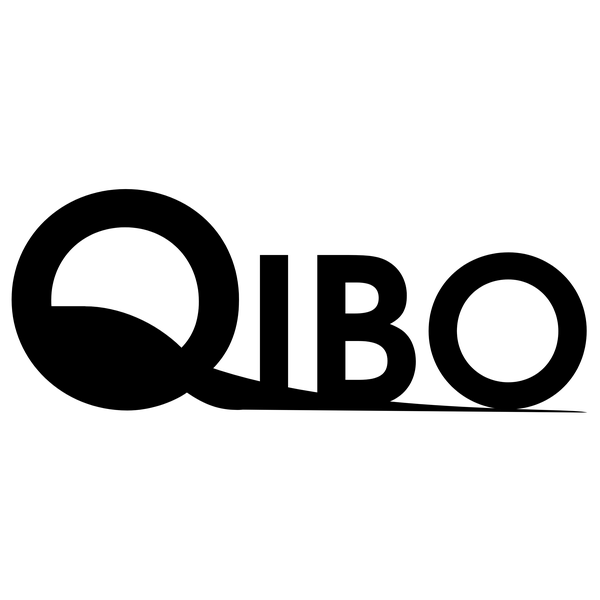
\includegraphics[width=.18\textwidth]{figures/qibo.png} 

\includegraphics[width=.18\textwidth]{figures/unimi.png} 

\includegraphics[width=.18\textwidth]{figures/cern.png}  

\includegraphics[width=.18\textwidth]{figures/qti.png}  
};
\end{tikzpicture}
}


\begin{document}

\maketitle

\begin{frame}{DALL-E 2 explaining my title}
\begin{figure}  
    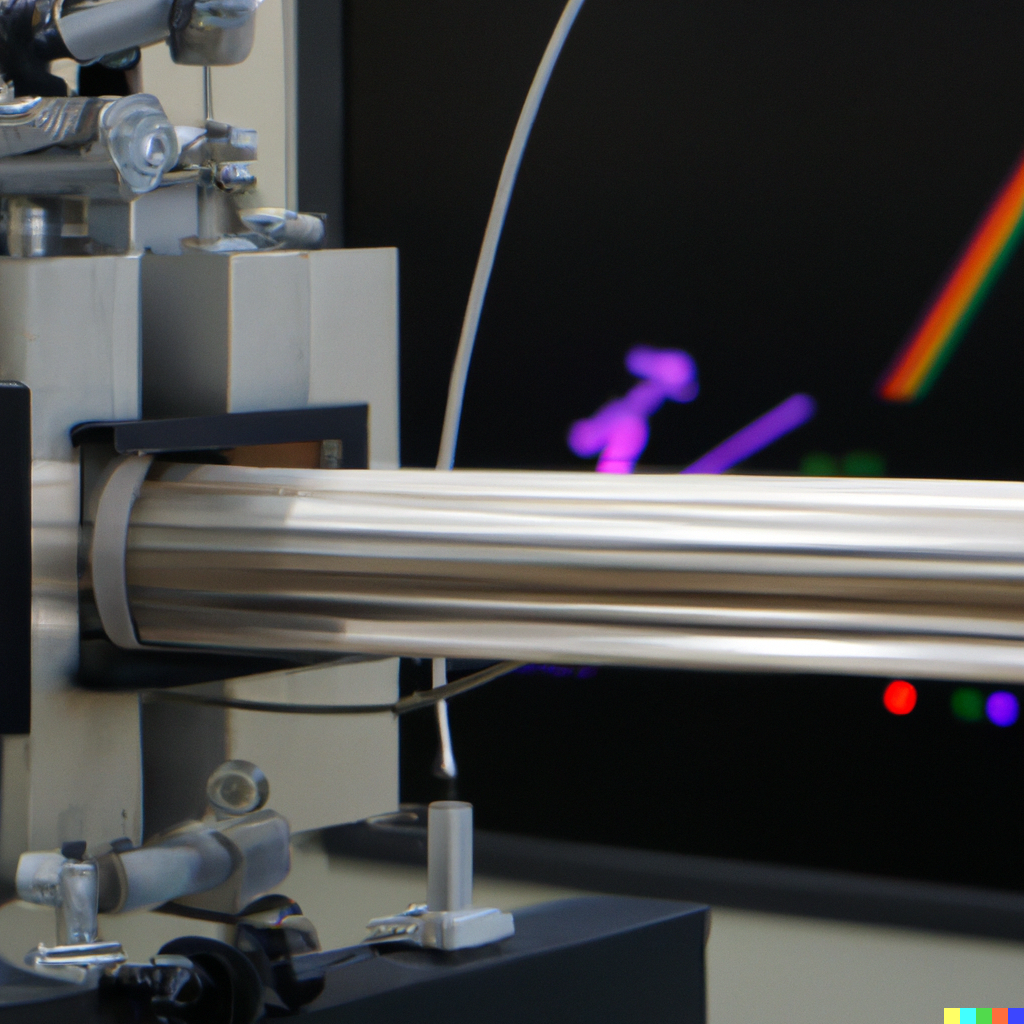
\includegraphics[width=0.35\textwidth]{figures/dalle1.png}%
    \,\,
    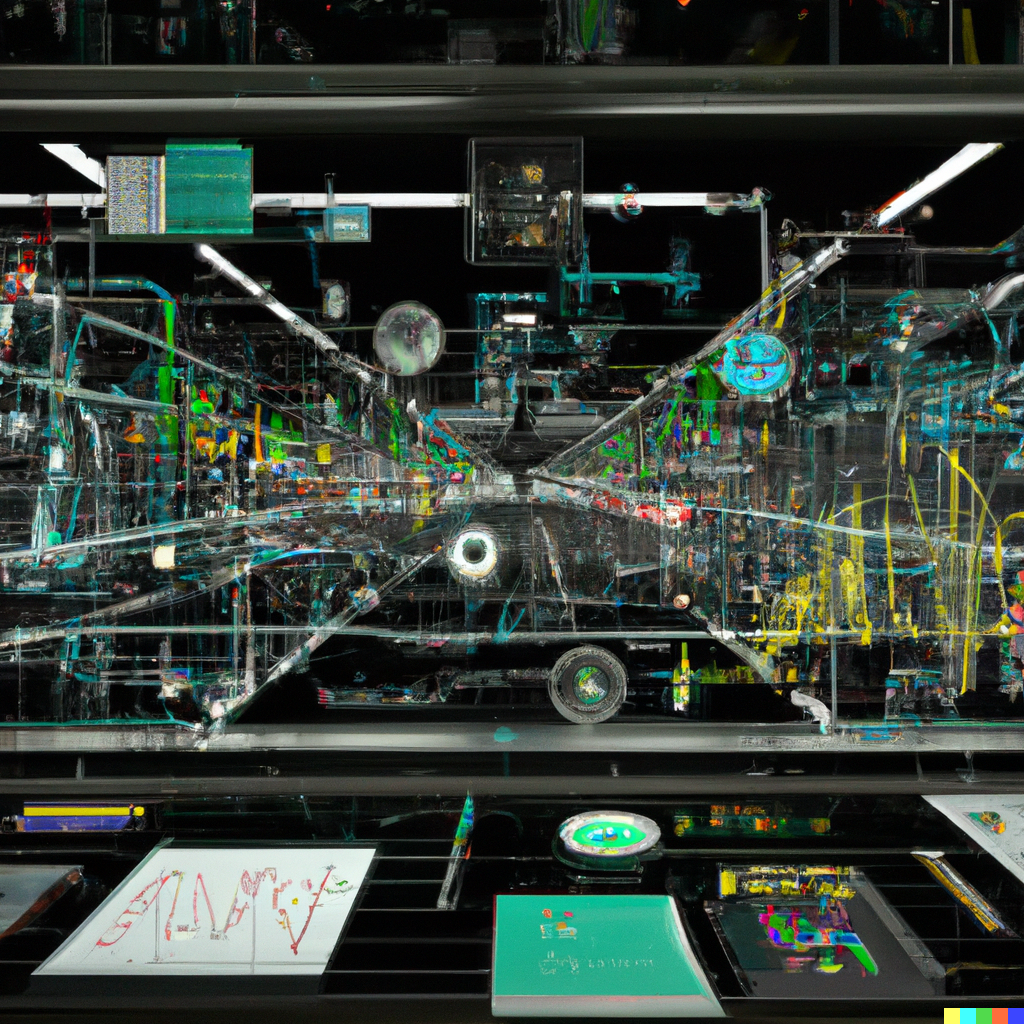
\includegraphics[width=0.35\textwidth]{figures/dalle2.png}

    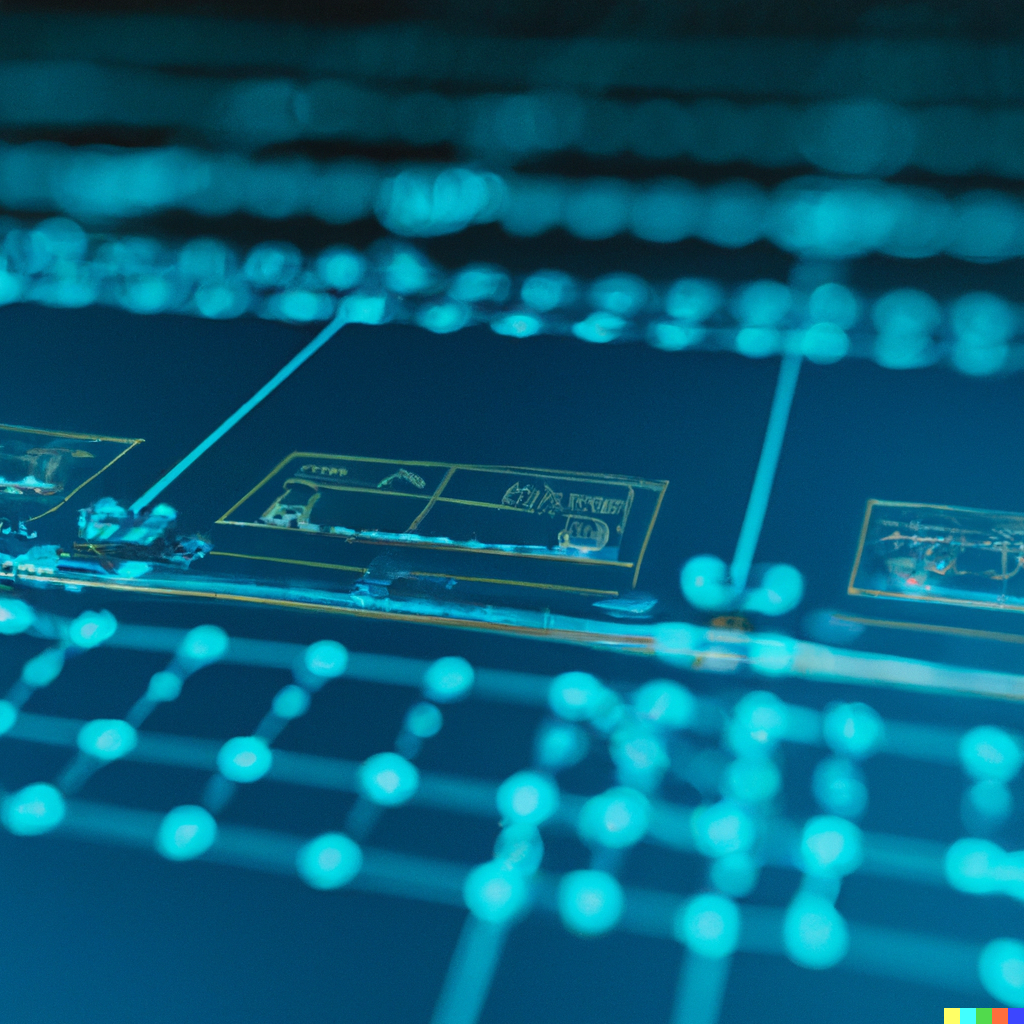
\includegraphics[width=0.35\textwidth]{figures/dalle3.png}%
    \,\,
    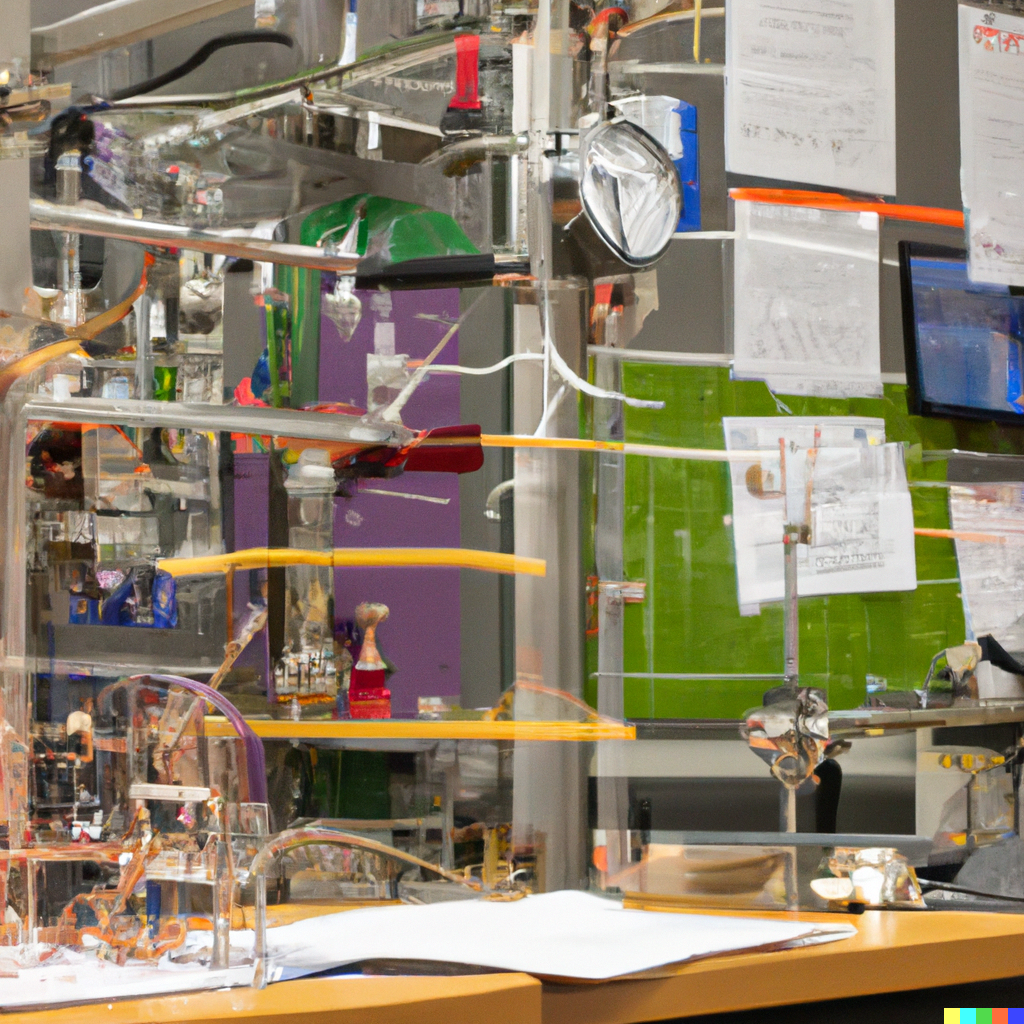
\includegraphics[width=0.35\textwidth]{figures/dalle4.png}
\end{figure}
\end{frame}


\begin{frame}{DALL-E 3 explaining my title}
\begin{figure}  
    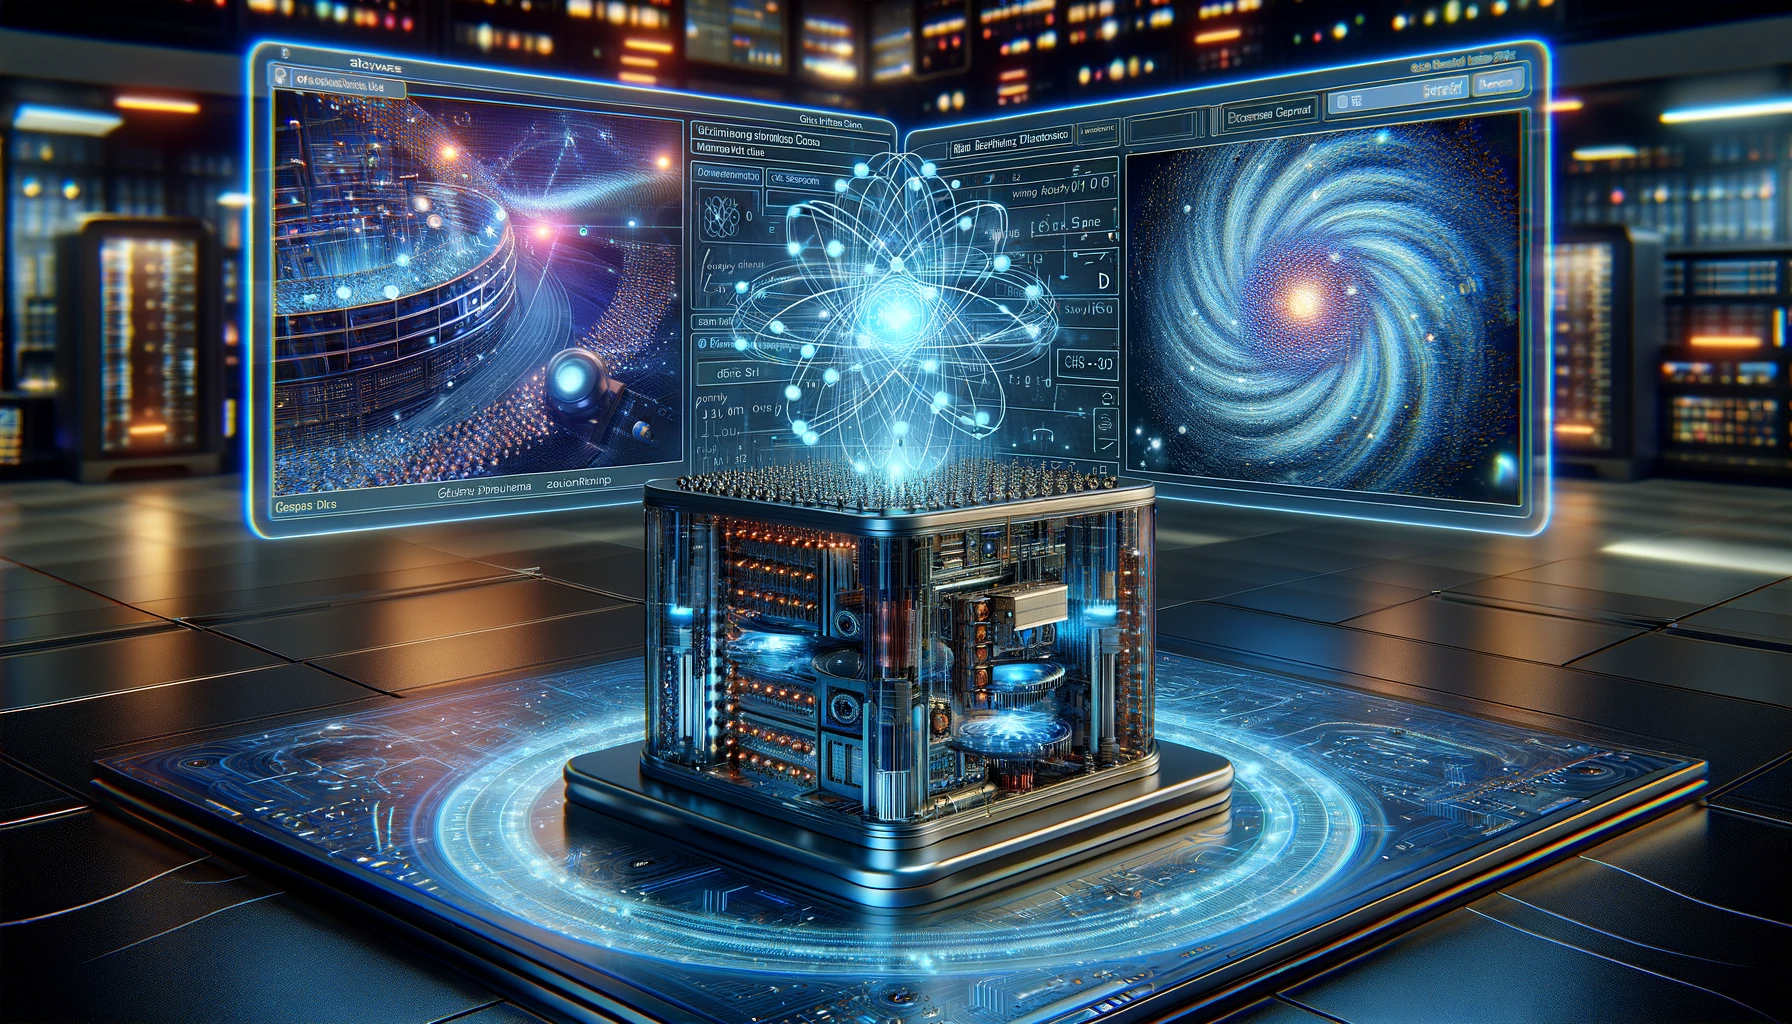
\includegraphics[width=1\textwidth]{figures/dalleplus.png}%
\end{figure}
\end{frame}

\begin{frame}{Me explaining my title}
\begin{figure}  
    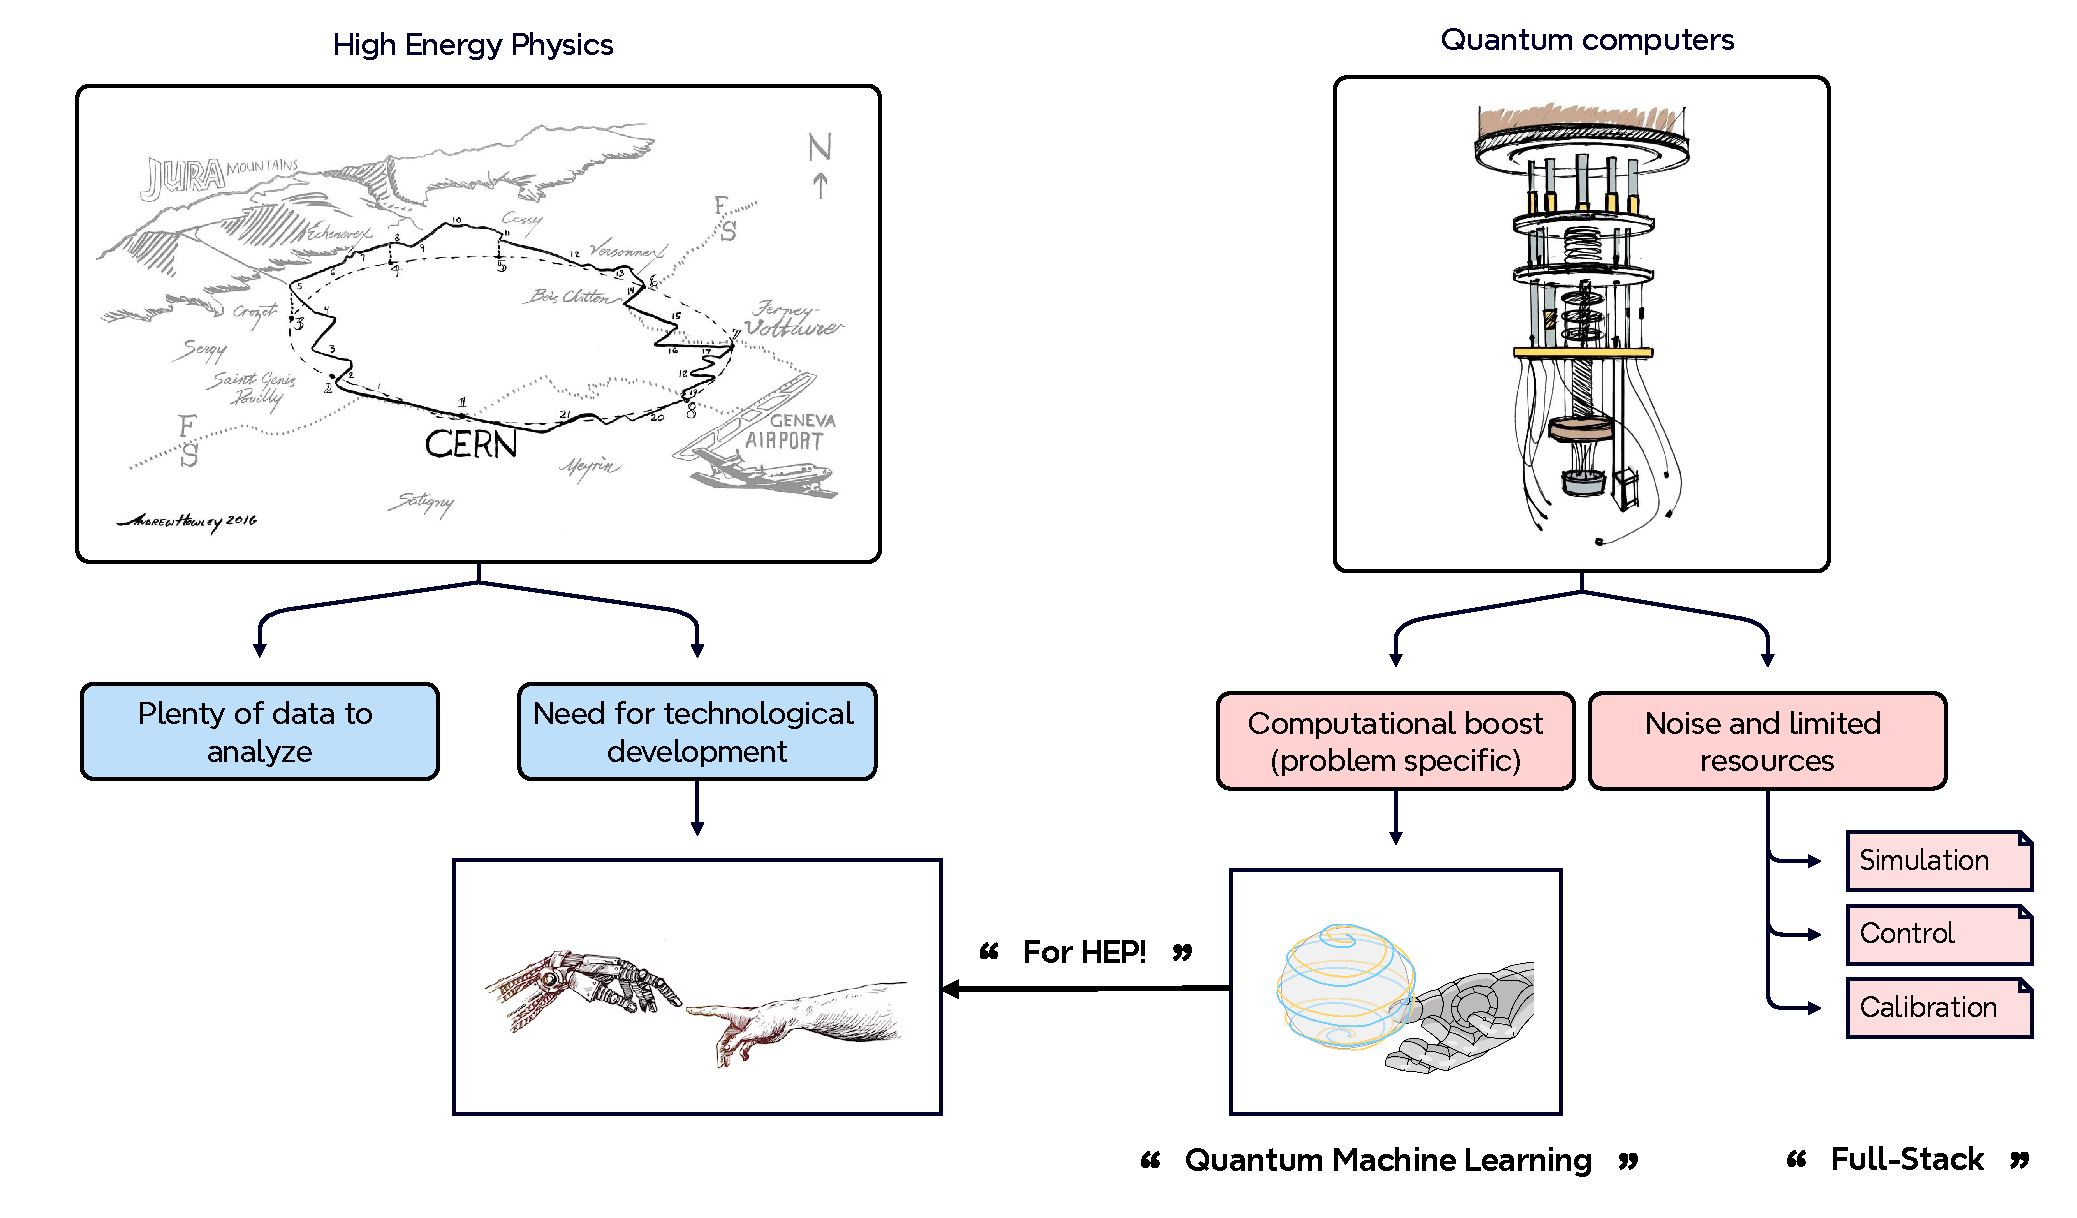
\includegraphics[width=1\textwidth]{figures/fsqml4hep}
\end{figure}
\end{frame}

\section{Introductory concepts}

\begin{frame}{Machine Learning (ML)}
\vspace{0.5cm}
ML helps in solving statistical problems, such as data generation, 
classification, etc.
\pause

Considering the supervised ML approach:
\pause
\begin{itemize}
\item[\faCrosshairs] we aim to know some hidden law between two variables: $\bm{y}=f(\bm{x})$;
\pause
\item[\faBarChart] we define a parameteric model which returns $\bm{y}_{\rm est}=f_{\rm est}(\bm{x}; \bm{\theta})$;
\pause
\item[\faBinoculars] we define an optimizer, which task is to compute 
   $\text{argmin}_{\bm{\theta}}\bigl[J(\bm{y}_{\rm meas}, \bm{y}_{\rm est})\bigr]$.
\end{itemize}
\pause
\vspace{-0.4cm}
\begin{figure}  
    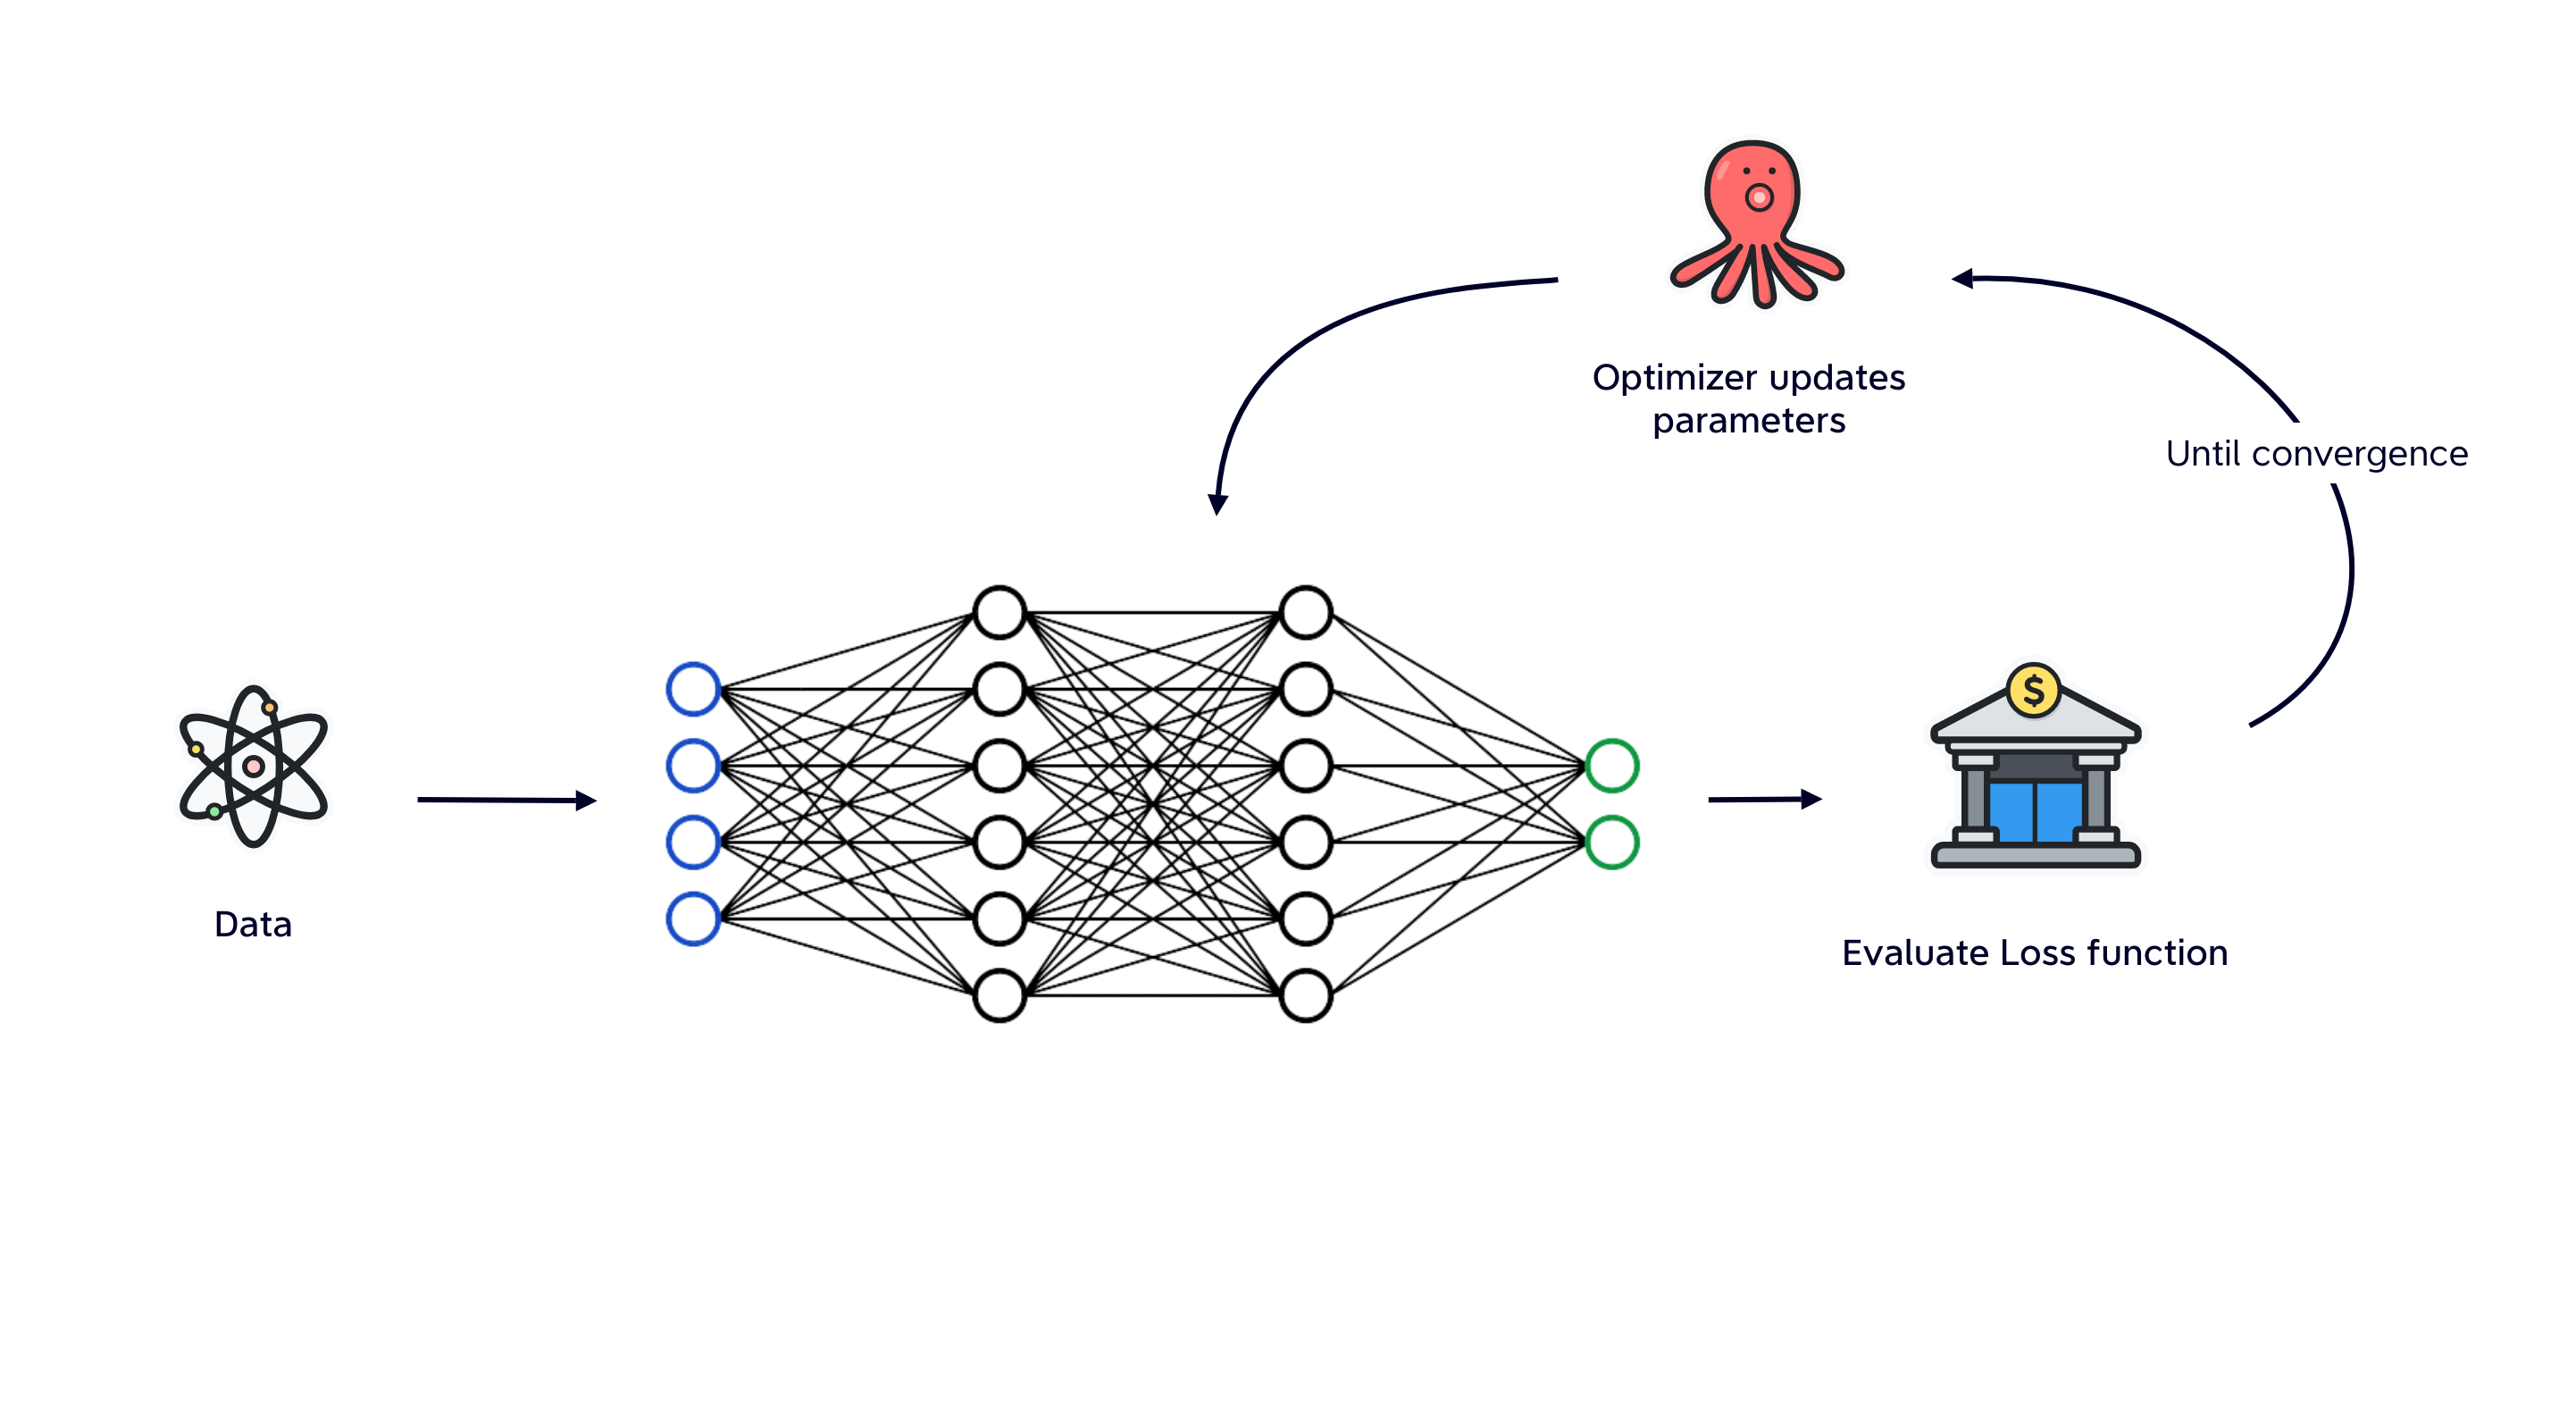
\includegraphics[width=1\textwidth]{figures/ml_scheme.png}
\end{figure}
\end{frame}

\begin{frame}{Qubits (on the Bloch sphere)}
\pause
Qubits' states can be used to process information:
\begin{equation*}
   \ket{\psi} = \alpha\ket{0}+\beta\ket{1} \qquad \text{where} \qquad \alpha = \cos{\frac{\theta}{2}}, \quad \beta = e^{i\phi}\sin{\frac{\theta}{2}}.
\end{equation*}
\begin{multicols}{2}
\def\rotationSphere{-110}
\def\radiusSphere{2cm}
\def\psiLat{45}
\def\psiLon{45}
\begin{blochsphere}[radius=\radiusSphere,opacity=0,rotation=\rotationSphere]
  % \drawBallGrid[style={opacity=.3}]{30}{45}
  % Draw the sphere...
  \drawLongitudeCircle[]{\rotationSphere}

  \drawLatitudeCircle[style={dashed}]{0}
  % Define the different points on the bloch sphere
  \labelLatLon{ket0}{90}{0};
  \labelLatLon{ket1}{-90}{0};
  \labelLatLon{ketminus}{0}{180};
  \labelLatLon{ketplus}{00}{0};
  \labelLatLon{ketpluspi2}{0}{-90};  % Longitude seems to be defined in the "wrong" direction, hence the minus
  \labelLatLon{ketplus3pi2}{0}{-270};
  \labelLatLon{psi}{\psiLat}{-\psiLon};
  % Draw and label the axis
  \draw[-latex] (0,0) -- (ket0) node[above,inner sep=.5mm] at (ket0) {\footnotesize $z$};
  \draw[-latex] (0,0) -- (ketplus) node[below,inner sep=.5mm] at (ketplus) {\footnotesize$x$};
  \draw[-latex] (0,0) -- (ketpluspi2) node[below,inner sep=.5mm] at (ketpluspi2) {\footnotesize $y$};
  % Draw |psi>
  \draw[-latex] (0,0) -- (psi) node[above]{\footnotesize $\ket{\psi}$};

  % Draw the angles
  \coordinate (origin) at (0,0);
  {
    % Will draw the angle/projection one the equatorial plane
    \setDrawingPlane{0}{0}
    % Draw the projection: cos is used to compute the length of the projection
    \draw[current plane,dashed] (0,0) -- (-90+\psiLon:{cos(\psiLat)*\radiusSphere}) coordinate (psiProjectedEquat) -- (psi);
    % Draw the angle
    \pic[current plane, draw,fill=purple!50,fill opacity=.5, text opacity=1,"\footnotesize $\phi$", angle eccentricity=2.2]{angle=ketplus--origin--psiProjectedEquat};
  }
  { \setLongitudinalDrawingPlane{\psiLon}
    % Draw the angle
    \pic[current plane, draw,fill=purple!50,fill opacity=.5, text opacity=1,"\footnotesize $\theta$", angle eccentricity=1.5]{angle=psi--origin--ket0};
  }
\end{blochsphere}

\pause

\def\rotationSphere{-110}
\def\radiusSphere{2cm}
\def\psiLat{45}
\def\psiLon{45}
\def\psiLatPrime{15} % Adjusted latitude for \psi' to be at the top
\def\psiLonPrime{-15} % Adjusted longitude for \psi' to be on the left-top

\begin{blochsphere}[radius=\radiusSphere, opacity=0, rotation=\rotationSphere]
  \drawLongitudeCircle[]{\rotationSphere}
  \drawLatitudeCircle[style={dashed}]{0}

  \labelLatLon{ket0}{90}{0};
  \labelLatLon{ket1}{-90}{0};
  \labelLatLon{ketminus}{0}{180};
  \labelLatLon{ketplus}{00}{0};
  \labelLatLon{ketpluspi2}{0}{-90};
  \labelLatLon{ketplus3pi2}{0}{-270};
  \labelLatLon{psi}{\psiLat}{-\psiLon};
  \labelLatLon{psiPrime}{\psiLatPrime}{-\psiLonPrime};

  \draw[-latex] (0,0) -- (ket0) node[above,inner sep=.5mm] at (ket0) {\footnotesize $z$};
  \draw[-latex] (0,0) -- (ketplus) node[below,inner sep=.5mm] at (ketplus) {\footnotesize$x$};
  \draw[-latex] (0,0) -- (ketpluspi2) node[below,inner sep=.5mm] at (ketpluspi2) {\footnotesize $y$};
  \draw[-latex, purple] (0,0) -- (psi) node[right, black]{\footnotesize $\ket{\psi}$};
  \draw[-latex, purple] (0,0) -- (psiPrime) node[left, black]{\footnotesize $\ket{\psi'}$};


% Draw modified trajectory with two curves before reaching psi'
\draw[purple, thick, ->] (psi) to[out=110, in=20] ++(-1,0.5) to[out=200, in=60] ++(0.3,-0.3) to[out=240, in=100] ++(-0.5,-0.3) to[out=280, in=100] (psiPrime);
\node[above left, purple] at ($(psi)!0.5!(psiPrime)$) {$\mathcal{U}$};
\end{blochsphere}
\end{multicols}
And this information can be manipulated applying unitaries $\mathcal{U}$. 
\end{frame}

\begin{frame}{Parametrized Quantum Circuits}
\pause
  \begin{itemize}
  \item<2,3,4,5>[\faMagic] Classical bits are replaced by \textbf{qubits}: 
  $\ket{\psi}=\alpha \ket{0} + \beta \ket{1}$;  
  \item<3,4,5>[\faCog] we modify the qubits state by applying unitaries, which can 
  be parametric $\mathcal{U}(\bm{\theta})$.
  \item<4,5>[\faBook] we call the unitaries \textbf{``gates''} and many gates together \textbf{``circuit''}.
  \item<5>[\faEye] after executing the circuit, information is accessed computing expectation values 
  of target observables on the new qubits state.
  \end{itemize}
    \begin{figure}
       \includegraphics<2>[width=0.8\textwidth]{figures/vqc_1.png}
       \includegraphics<3,4>[width=0.8\textwidth]{figures/vqc_2.png}
       \includegraphics<5>[width=0.8\textwidth]{figures/vqc.png}   
    \end{figure}
\end{frame}

% SLIDE 1 QML
\begin{frame}{Quantum Machine Learning - doing ML using QC}

\vspace{1.05cm}

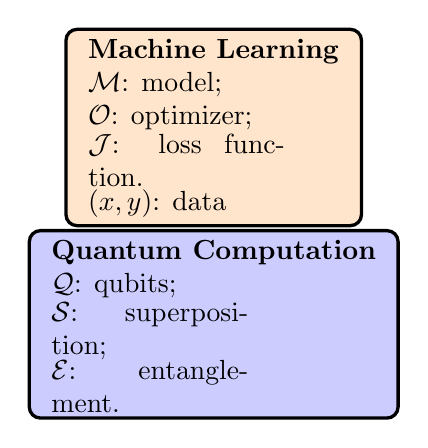
\begin{tikzpicture}[->,>=stealth']

 \node[state, fill=orange!20] (ML) 
 {\begin{tabular}{l}
 \textbf{Machine Learning}\\ 
 \parbox{2.5cm}{$\mathcal{M}$: model;}\\
 \parbox{2.5cm}{$\mathcal{O}$: optimizer;}\\
 \parbox{2.5cm}{$\mathcal{J}$: loss function.}\\
 \parbox{2.5cm}{$(x, y)$: data}
  \end{tabular}
  };
  
  \node[state,
  below of = ML,
  yshift=-1.5cm, fill=blue!20] (QC) 
 {\begin{tabular}{l}
 \textbf{Quantum Computation}\\ 
 \parbox{2.5cm}{$\mathcal{Q}$: qubits;} \\
 \parbox{2.5cm}{$\mathcal{S}$: superposition;}\\
 \parbox{2.5cm}{$\mathcal{E}$: entanglement.}
  \end{tabular}
  };
  
\end{tikzpicture}
\end{frame}


% SLIDE 2 QML
\begin{frame}{Quantum Machine Learning - operating on qubits}

\vspace{1.77cm}

\begin{tikzpicture}[->,>=stealth']

 \node[state, fill=orange!20] (ML) 
 {\begin{tabular}{l}
 \textbf{Machine Learning}\\ 
 \parbox{2.5cm}{$\mathcal{M}$: model;}\\
 \parbox{2.5cm}{$\mathcal{O}$: optimizer;}\\
 \parbox{2.5cm}{$\mathcal{J}$: loss function.}\\
 \parbox{2.5cm}{$(x, y)$: data}
  \end{tabular}
  };
  
  \node[state,
  below of = ML,
  yshift=-1.5cm, fill=blue!20] (QC) 
 {\begin{tabular}{l}
 \textbf{Quantum Computation}\\ 
 \parbox{2.5cm}{$\mathcal{Q}$: qubits;} \\
 \parbox{2.5cm}{$\mathcal{S}$: superposition;}\\
 \parbox{2.5cm}{$\mathcal{E}$: entanglement.}
  \end{tabular}
  };
  
 \node[state,
    right of=QC,
    yshift=-0.5cm,
    anchor=center,
    node distance=4.5cm, 	
    text width=3.5cm, fill=blue!20] (VQC) 
 {%
 \begin{tabular}{l}
  \textbf{Circuit execution} \\
  \parbox{4.5cm}{
  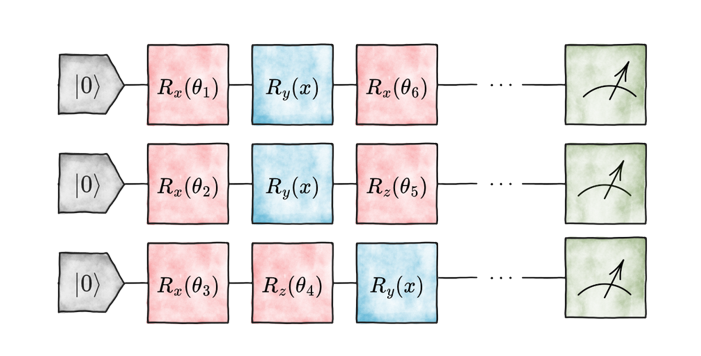
\includegraphics[width=0.9\textwidth]{figures/vqc.png}
  }
 \end{tabular}
 };
 
  \draw[line width=0.3mm] (1, -2.5)  to[out=0, in=200] (3, -3.2);
\end{tikzpicture}

\end{frame}

% SLIDE 3 QML
\begin{frame}{Quantum Machine Learning - natural randomness}

\vspace{1.77cm}

\begin{tikzpicture}[->,>=stealth']

 \node[state, fill=orange!20] (ML) 
 {\begin{tabular}{l}
 \textbf{Machine Learning}\\ 
 \parbox{2.5cm}{$\mathcal{M}$: model;}\\
 \parbox{2.5cm}{$\mathcal{O}$: optimizer;}\\
 \parbox{2.5cm}{$\mathcal{J}$: loss function.}\\
 \parbox{2.5cm}{$(x, y)$: data}
  \end{tabular}
  };
  
  \node[state,
  below of = ML,
  yshift=-1.5cm, fill=blue!20] (QC) 
 {\begin{tabular}{l}
 \textbf{Quantum Computation}\\ 
 \parbox{2.5cm}{$\mathcal{Q}$: qubits;} \\
 \parbox{2.5cm}{$\mathcal{S}$: superposition;}\\
 \parbox{2.5cm}{$\mathcal{E}$: entanglement.}
  \end{tabular}
  };
  
 \node[state,
    right of=QC,
    yshift=-0.5cm,
    anchor=center,
    node distance=4.5cm, 	
    text width=3.5cm, fill=blue!20] (VQC) 
 {%
 \begin{tabular}{l}
  \textbf{Circuit execution} \\
  \parbox{4.5cm}{
  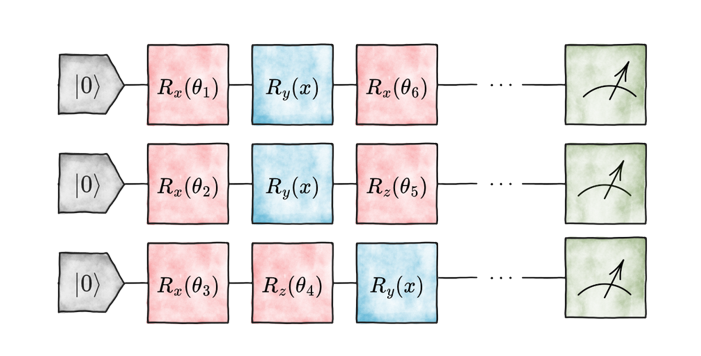
\includegraphics[width=0.9\textwidth]{figures/vqc.png}
  }
 \end{tabular}
 };
 
\node[state,
  right of = VQC,
  node distance = 3cm,
  yshift=2cm, 
  fill=blue!20] (NSHOT) 
 {\begin{tabular}{l}
 \textbf{Expected values}\\ 
 $y_{est} \equiv \braket{\psi'|\hat{O}|\psi'}$
  \end{tabular}
  };
 
\draw[line width=0.3mm] (1, -2.5)  to[out=0, in=200] (3, -3.2);
\draw[line width=0.3mm] (6, -2.8)  to[out=0, in=250] (7, -1.6);
\end{tikzpicture}

\end{frame}


% SLIDE 4 QML
\begin{frame}{Quantum Machine Learning - encoding the problem}

\vspace{0.56cm}
\begin{tikzpicture}[->,>=stealth']

 \node[state, fill=orange!20] (ML) 
 {\begin{tabular}{l}
 \textbf{Machine Learning}\\ 
 \parbox{2.5cm}{$\mathcal{M}$: model;}\\
 \parbox{2.5cm}{$\mathcal{O}$: optimizer;}\\
 \parbox{2.5cm}{$\mathcal{J}$: loss function.}\\
 \parbox{2.5cm}{$(x, y)$: data}
  \end{tabular}
  };
  
  \node[state,
  below of = ML,
  yshift=-1.5cm, fill=blue!20] (QC) 
 {\begin{tabular}{l}
 \textbf{Quantum Computation}\\ 
 \parbox{2.5cm}{$\mathcal{Q}$: qubits;} \\
 \parbox{2.5cm}{$\mathcal{S}$: superposition;}\\
 \parbox{2.5cm}{$\mathcal{E}$: entanglement.}
  \end{tabular}
  };
  
 
 \node[state,
    right of=QC,
    yshift=-0.5cm,
    anchor=center,
    node distance=4.5cm, 	
    text width=3.5cm, fill=blue!20] (VQC) 
 {%
 \begin{tabular}{l}
  \textbf{Circuit execution} \\
  \parbox{4.5cm}{
  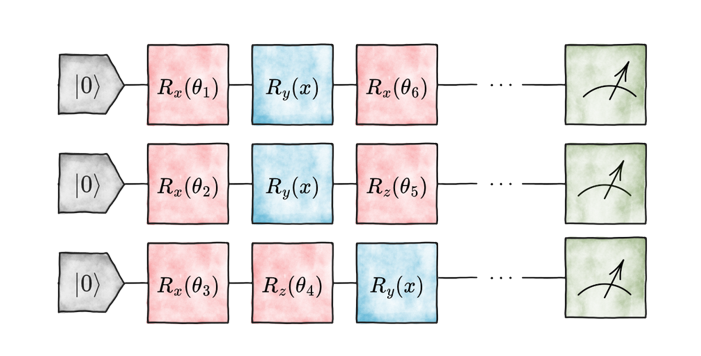
\includegraphics[width=0.9\textwidth]{figures/vqc.png}
  }
 \end{tabular}
 };
 
\node[state,
  right of = VQC,
  node distance = 3cm,
  yshift=2cm, 
  fill=blue!20] (NSHOT) 
 {\begin{tabular}{l}
 \textbf{Expected values}\\ 
 $y_{est} \equiv \braket{\psi'|\hat{O}|\psi'}$
  \end{tabular}
  };

  
 \draw[line width=0.3mm, red, opacity = 0.7] (0.5, 0.4)  to[out=0, in=230] (3, -3.3);
 \draw[line width=0.3mm, orange, opacity = 0.7] (-1.2, -1.25)  to[out=260, in=300] (4.4, -4.1);
 \draw[line width=0.3mm, cadmiumgreen, opacity = 0.7] (-0.4, -1.2)  to[out=330, in=80] (7.8, -0.4);
  
 
 \draw[red, line width=0.4mm, opacity = 0.9] (-1.1, 0.4) circle (0.4 cm);
 \draw[cadmiumgreen, line width=0.4mm, opacity = 0.9] (-0.65,-0.8) circle (0.3 cm);
 \draw[cadmiumgreen, line width=0.4mm, opacity = 0.9] (7.2,-1.4) rectangle (8.6, -0.95);
 \draw[orange, line width=0.4mm, opacity = 0.6] (-1.15,-0.8) circle (0.3 cm);
 \draw[red, line width=0.4mm, opacity = 0.6] (3.1,-4) rectangle (6,-2.4);
 \draw[orange, line width=0.4mm, opacity = 0.9] (3.5,-3.9) rectangle (5.2,-2.5);


\end{tikzpicture}
\end{frame}


% SLIDE 5 QML
\begin{frame}{Quantum Machine Learning!}

\vspace{0.42cm}
\begin{tikzpicture}[->,>=stealth']


 \node[state, fill=orange!20] (ML) 
 {\begin{tabular}{l}
 \textbf{Machine Learning}\\ 
 \parbox{2.5cm}{$\mathcal{M}$: model;}\\
 \parbox{2.5cm}{$\mathcal{O}$: optimizer;}\\
 \parbox{2.5cm}{$\mathcal{J}$: loss function.}\\
 \parbox{2.5cm}{$(x, y)$: data}
  \end{tabular}
  };
  
  \node[state,
  below of = ML,
  yshift=-1.5cm, fill=blue!20] (QC) 
 {\begin{tabular}{l}
 \textbf{Quantum Computation}\\ 
 \parbox{2.5cm}{$\mathcal{Q}$: qubits;} \\
 \parbox{2.5cm}{$\mathcal{S}$: superposition;}\\
 \parbox{2.5cm}{$\mathcal{E}$: entanglement.}
  \end{tabular}
  };
  

 \node[state,   
  text width=3cm, 
  yshift=1.5cm, 
  right of=ML, 	
  node distance=4cm, 
  anchor=center, fill=green!20] (OPT) 
 {%
 \begin{tabular}{l} 	% content
  \textbf{Optimizer $\mathcal{O}$}\\
  Hybrid-strategy
 \end{tabular}
 };
 
 \node[state,
    right of=QC,
    yshift=-0.5cm,
    anchor=center,
    node distance=4.5cm, 	
    text width=3.5cm, fill=blue!20] (VQC) 
 {%
 \begin{tabular}{l}
  \textbf{Circuit execution} \\
  \parbox{4.5cm}{
  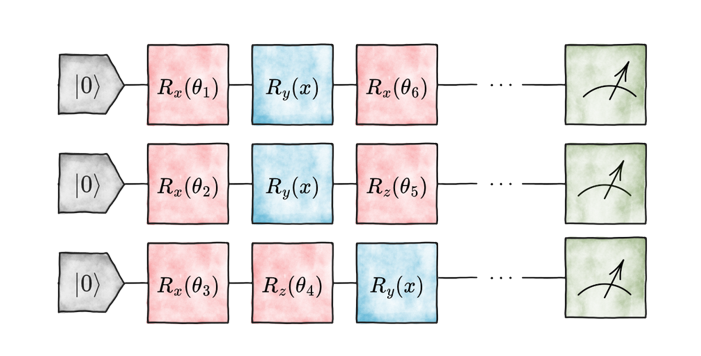
\includegraphics[width=0.9\textwidth]{figures/vqc.png}
  }
 \end{tabular}
 };
 
\node[state,
  right of = VQC,
  node distance = 3cm,
  yshift=2cm, 
  fill=blue!20] (NSHOT) 
 {\begin{tabular}{l}
 \textbf{Expected values}\\ 
 $y_{est} \equiv \braket{\psi'|\hat{O}|\psi'}$
  \end{tabular}
  };
  
  \node[state,
  above of = NSHOT,
  node distance = 1.5cm,
  yshift=0cm, fill=green!20] (J) 
 {\begin{tabular}{l}
 \textbf{loss function $\mathcal{J}$}\\ 
 $\mathcal{J}(y_{meas}, y_{est})$
  \end{tabular}
  };
  

 \draw[line width=0.3mm] (6.5, -3)  to[out=0, in=270] (7.5, -1.6);
 \draw[line width=0.3mm] (6, -1.1)  to[out=180, in=200] (6.1, 0.2);
 \draw[line width=0.3mm] (7.5, 1.1)  to[out=90, in=0] (5.7, 1.5);
 \draw[line width=0.6mm, opacity=0.8] (2, 1.6)  to[out=180, in=270] (-0.2, 2.9);
 
 \draw[line width=0.3mm, orange, opacity = 0.0] (-1.2, -1.25)  to[out=260, in=300] (4.4, -3.5);

\end{tikzpicture}
\end{frame}

\begin{frame}{From ML to QML}
\begin{figure}  
   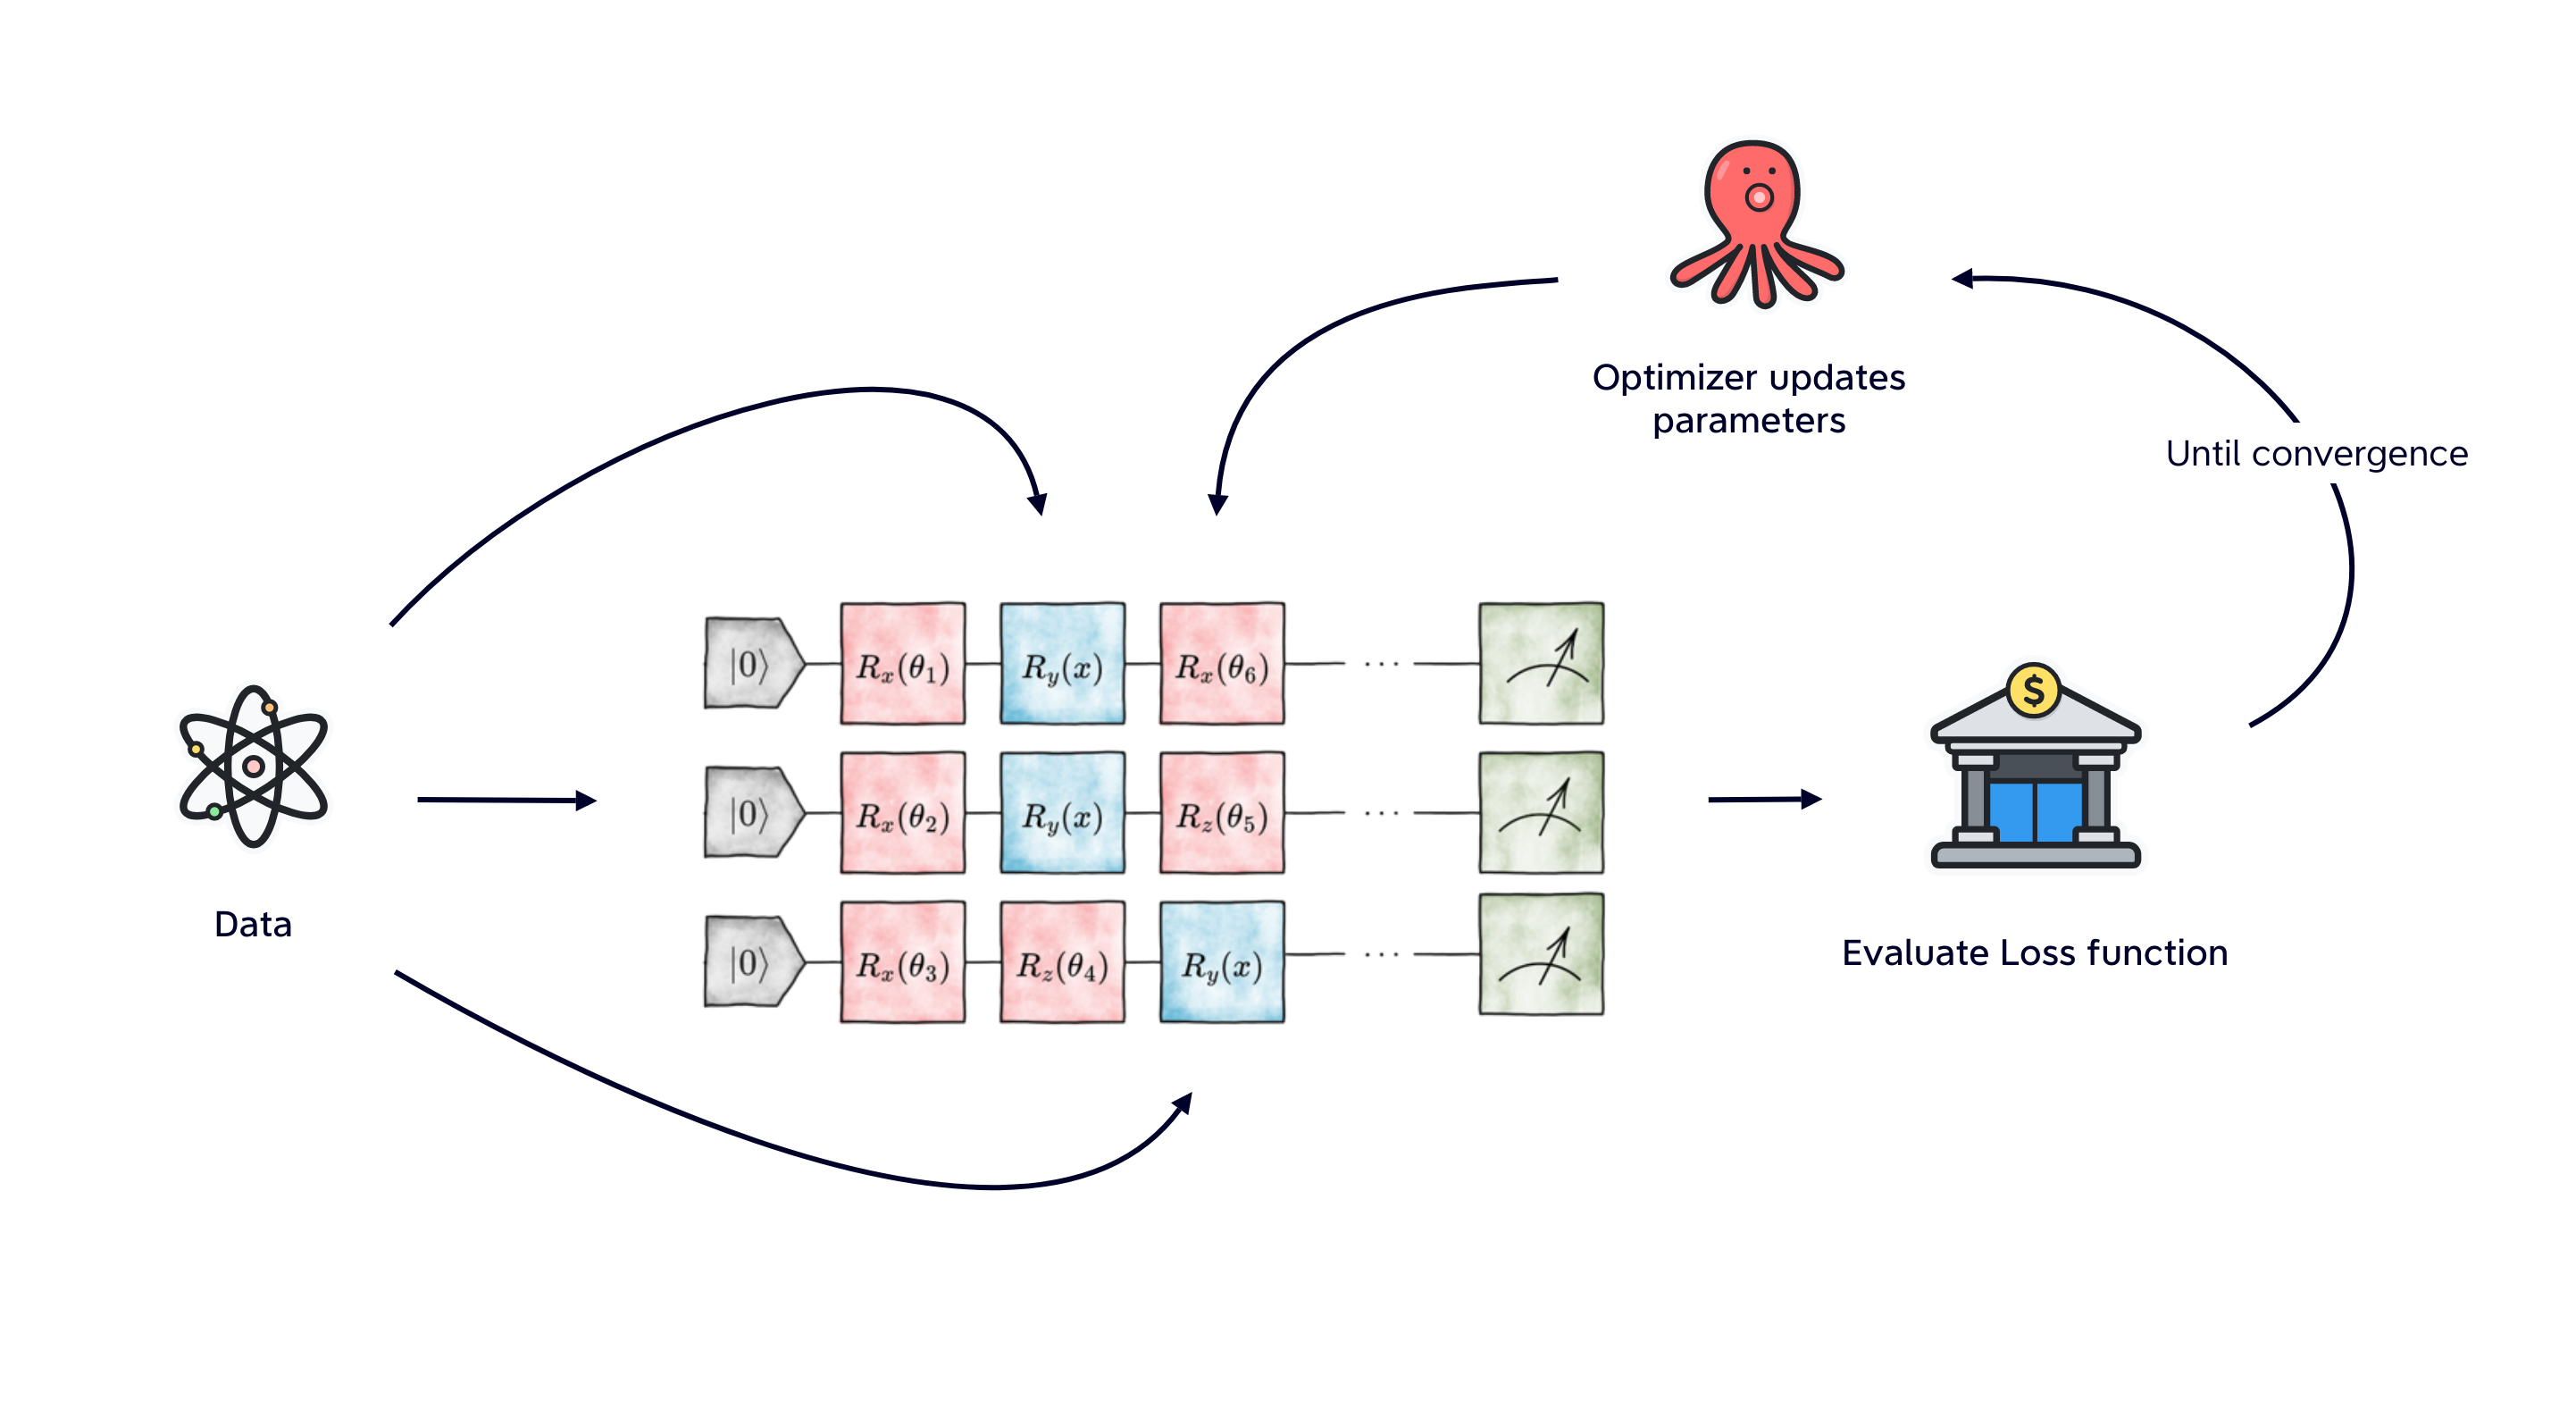
\includegraphics[width=1\textwidth]{figures/qml_scheme.png}
\end{figure}
\end{frame}

\begin{frame}{Why QML?}
\begin{multicols}{2}
\begin{itemize}
\item<2,3,4,5,6,7>[\faCartPlus] we collect \textbf{high-dimensional} data, which challenge classical models;
\item<3,4,5,6,7>[\faCodepen] an $N$-long input variable can be stored in a $\log{N}$ qubits system; 
\item<4,5,6,7>[\faLeaf ] low power consuption\only<4->{\footnote{\faBook\,\,
\href{https://doi.org/10.1038/s43588-023-00459-6}{\textit{Are quantum computers really energy efficient?}, Sophia Chen, Jun 2023}}};
\item<5,6,7>[\faCut] can \textbf{superposition} and \textbf{entanglement} be exploited to use less 
\textbf{parameters}?
\item<6,7>[\faUserSecret ] can superposition and entanglement better deal with quantum data?\only<6->{\footnote{\faBook\,\,
\href{https://arxiv.org/abs/2307.03236}{\textit{Quantum Computing for High-Energy 
Physics: State of the Art and Challenges}, A. Di Meglio et al., Jul 2023}}}\only<6->{\footnote{\faBook\,\,
\href{https://arxiv.org/abs/2307.03236}{\textit{Quantum anomaly detection in the 
latent space of proton collision events at the LHC}, K. A. Woźniak et al., Jan 2023}}}
\end{itemize}
\begin{figure}  
   \uncover<7->{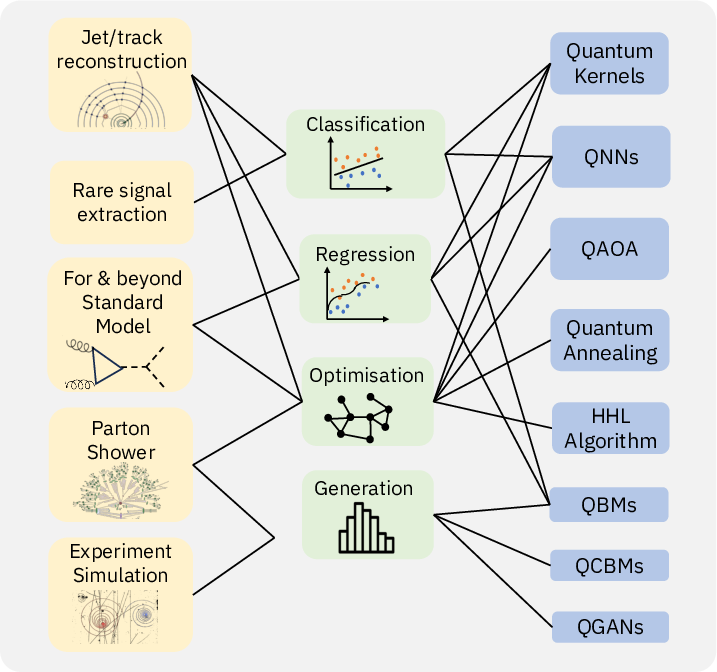
\includegraphics[width=0.5\textwidth]{figures/HEP_utils.png}}
\end{figure}
\end{multicols}
\only<2-3>{\vspace{0.8cm}}
\only<4-5>{\vspace{0.57cm}}
\end{frame}

\begin{frame}{My playground: \texttt{Qibo}}
\begin{figure}  
   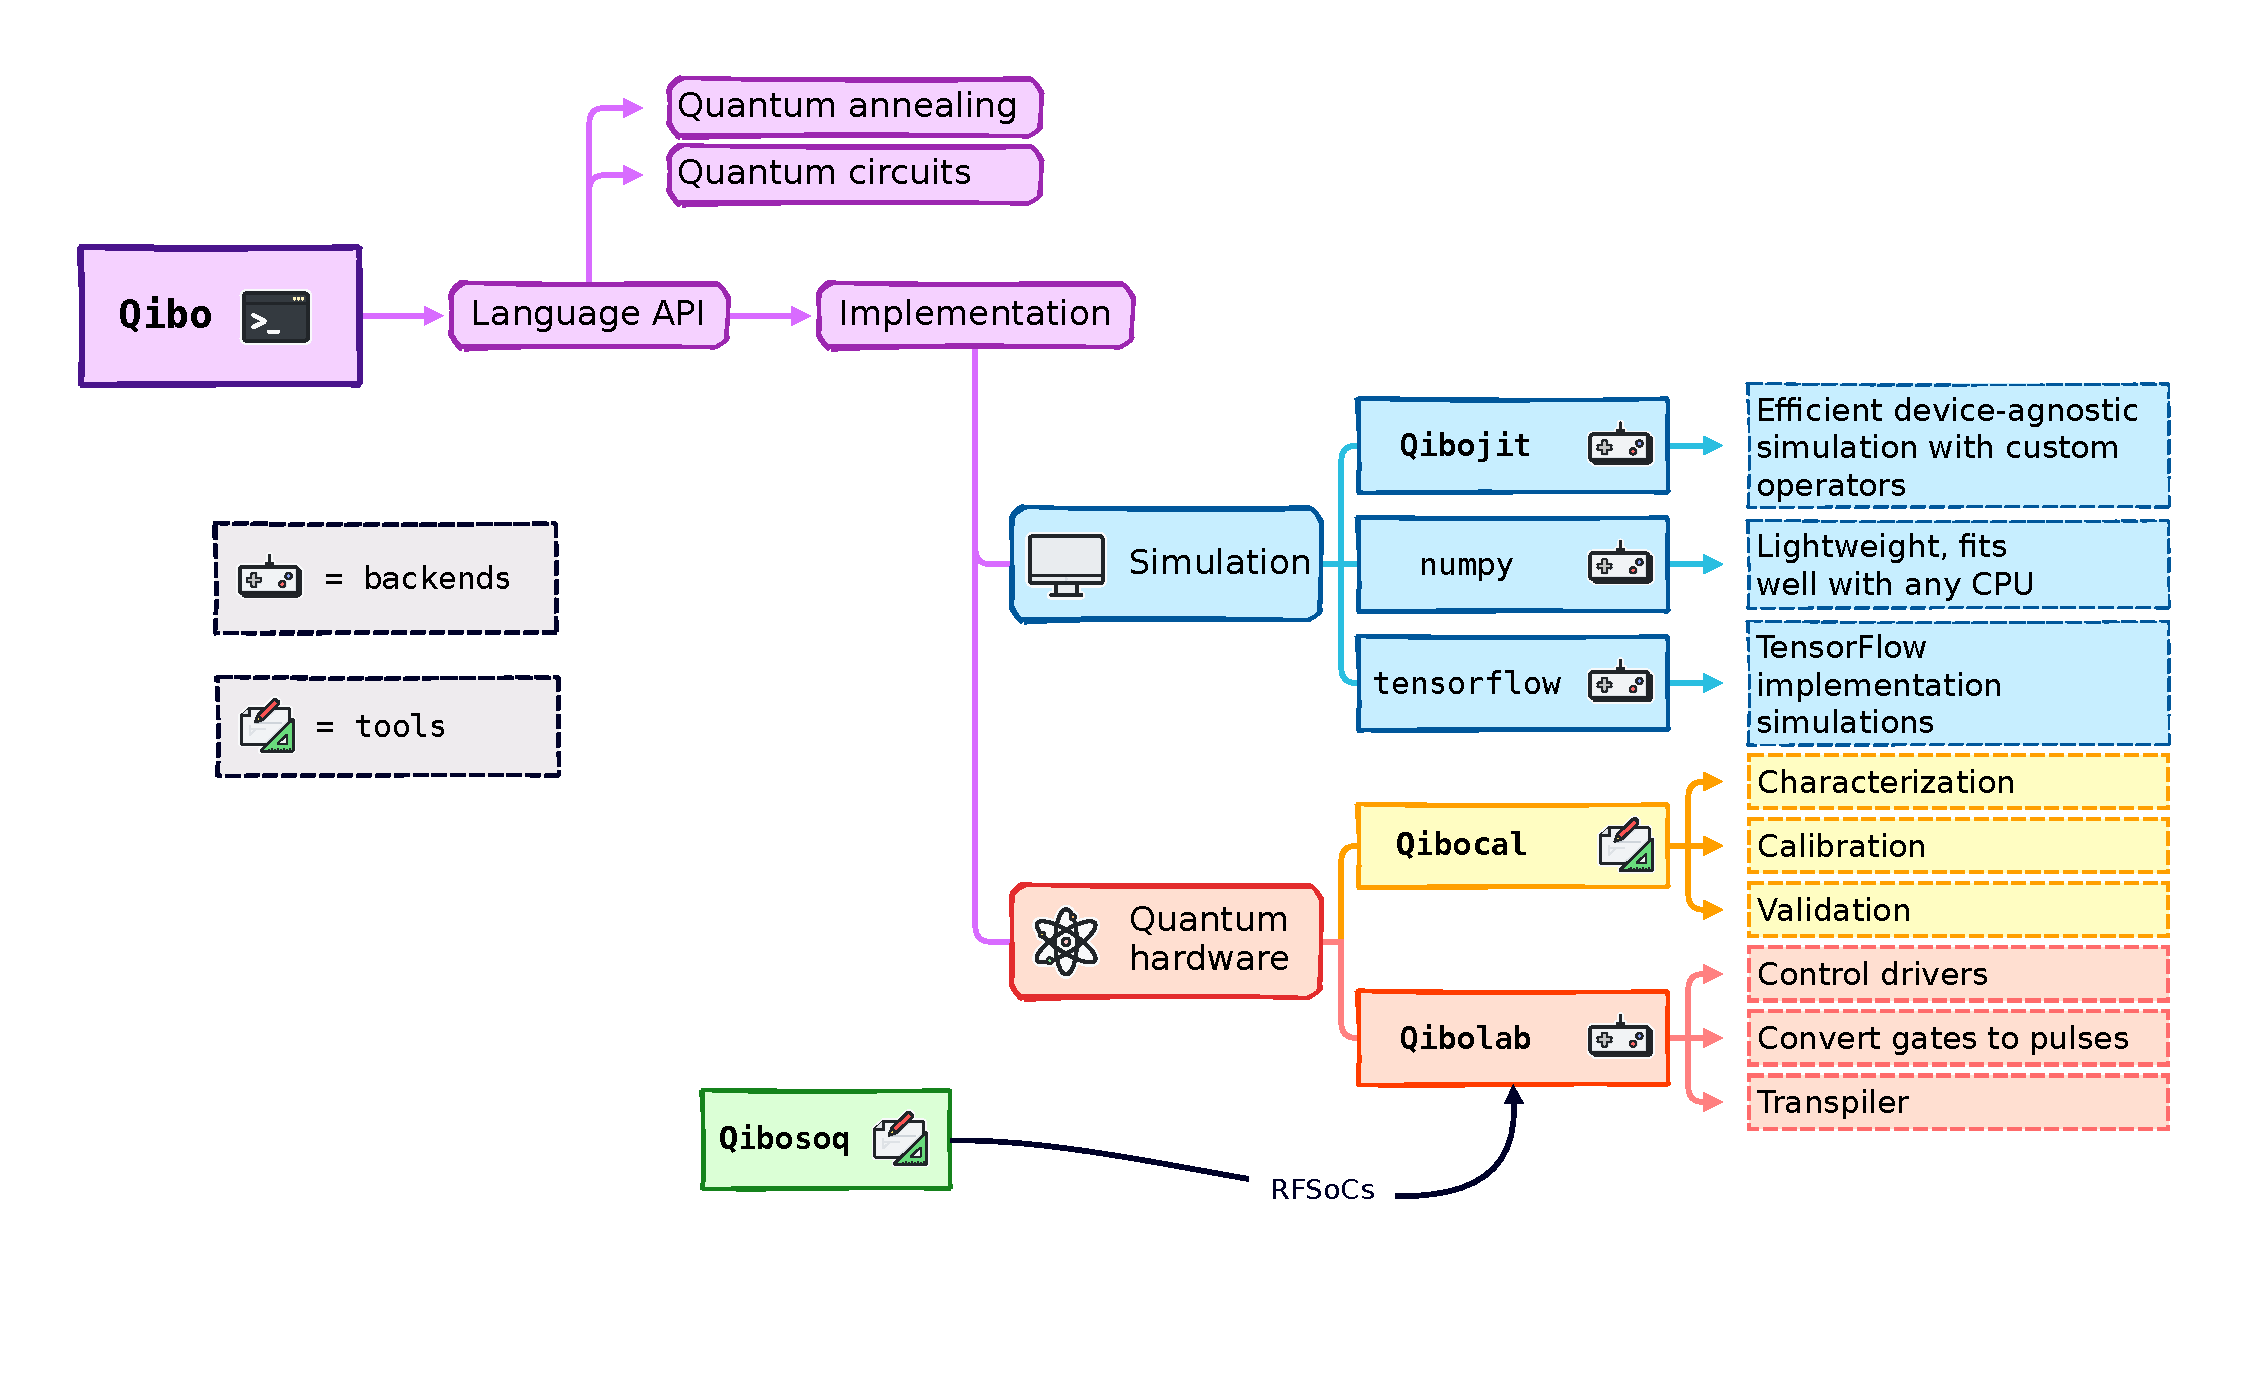
\includegraphics[width=1\textwidth]{figures/qibo_ecosystem.pdf}
\end{figure}
\end{frame}

\begin{frame}{My playground: \texttt{Qibo}}
\begin{figure}  
   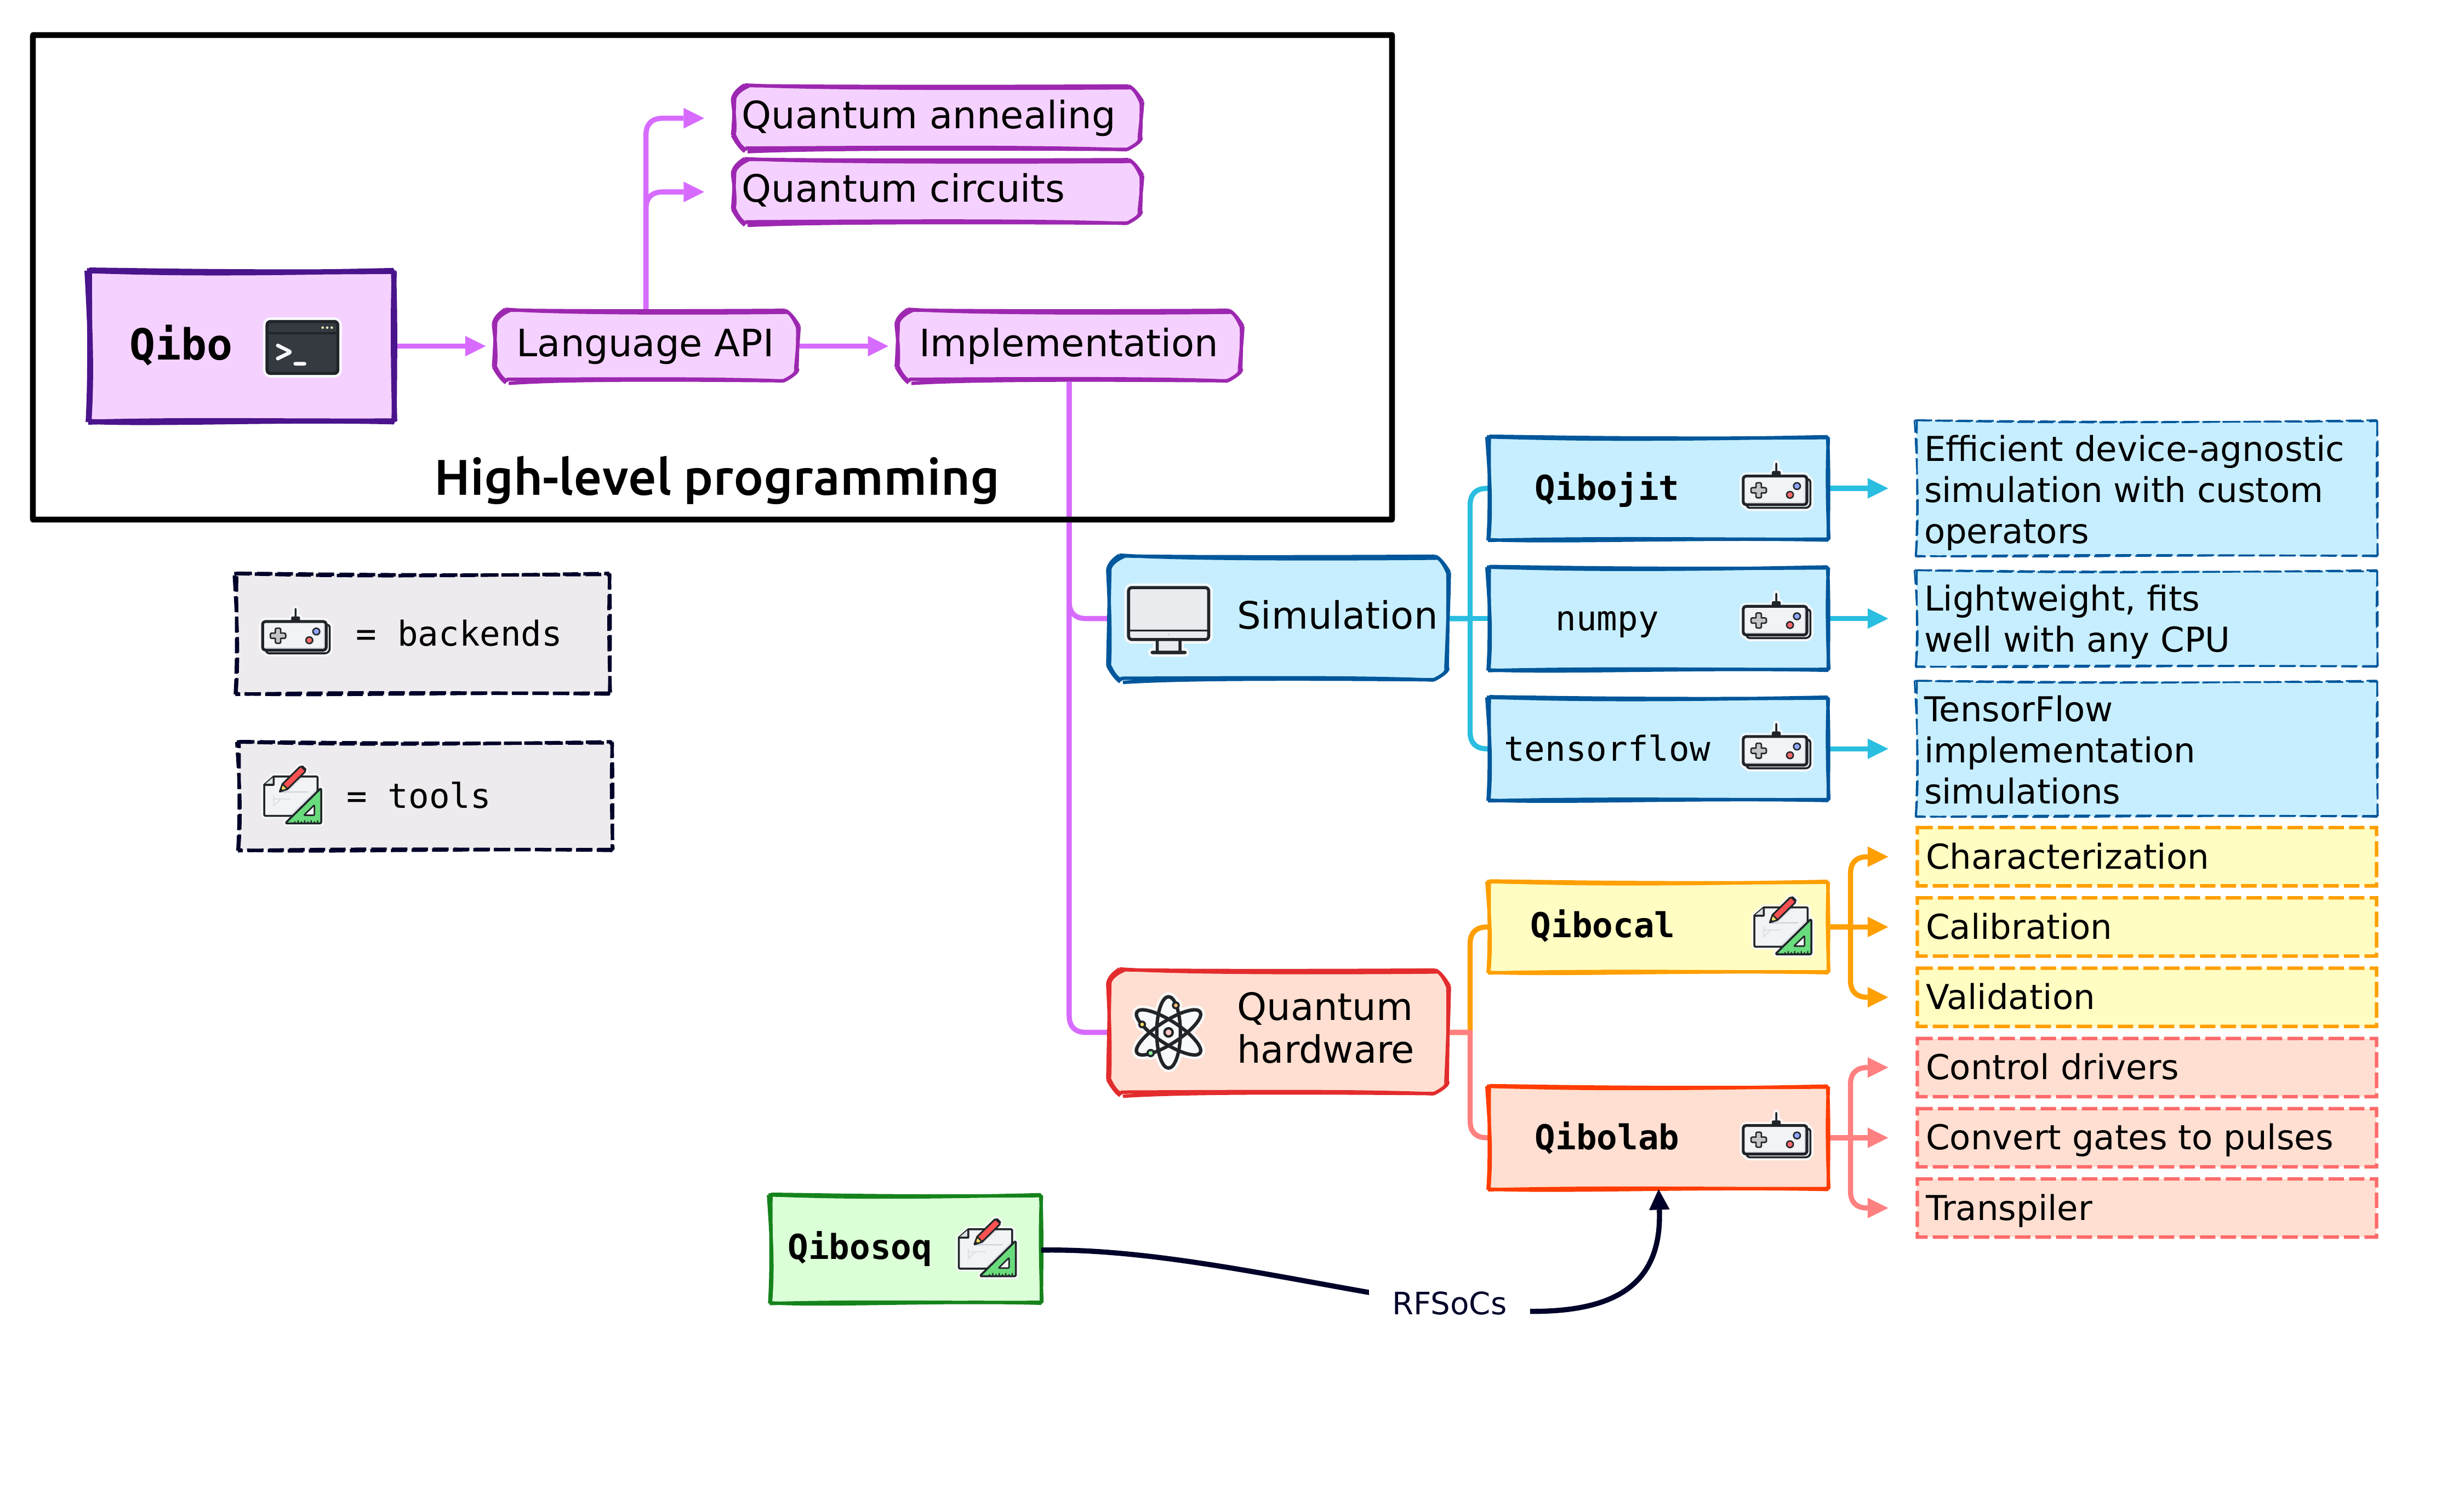
\includegraphics[width=1\textwidth]{figures/eco1.png}
\end{figure}
\end{frame}

\begin{frame}{My playground: \texttt{Qibo}}
\begin{figure}  
   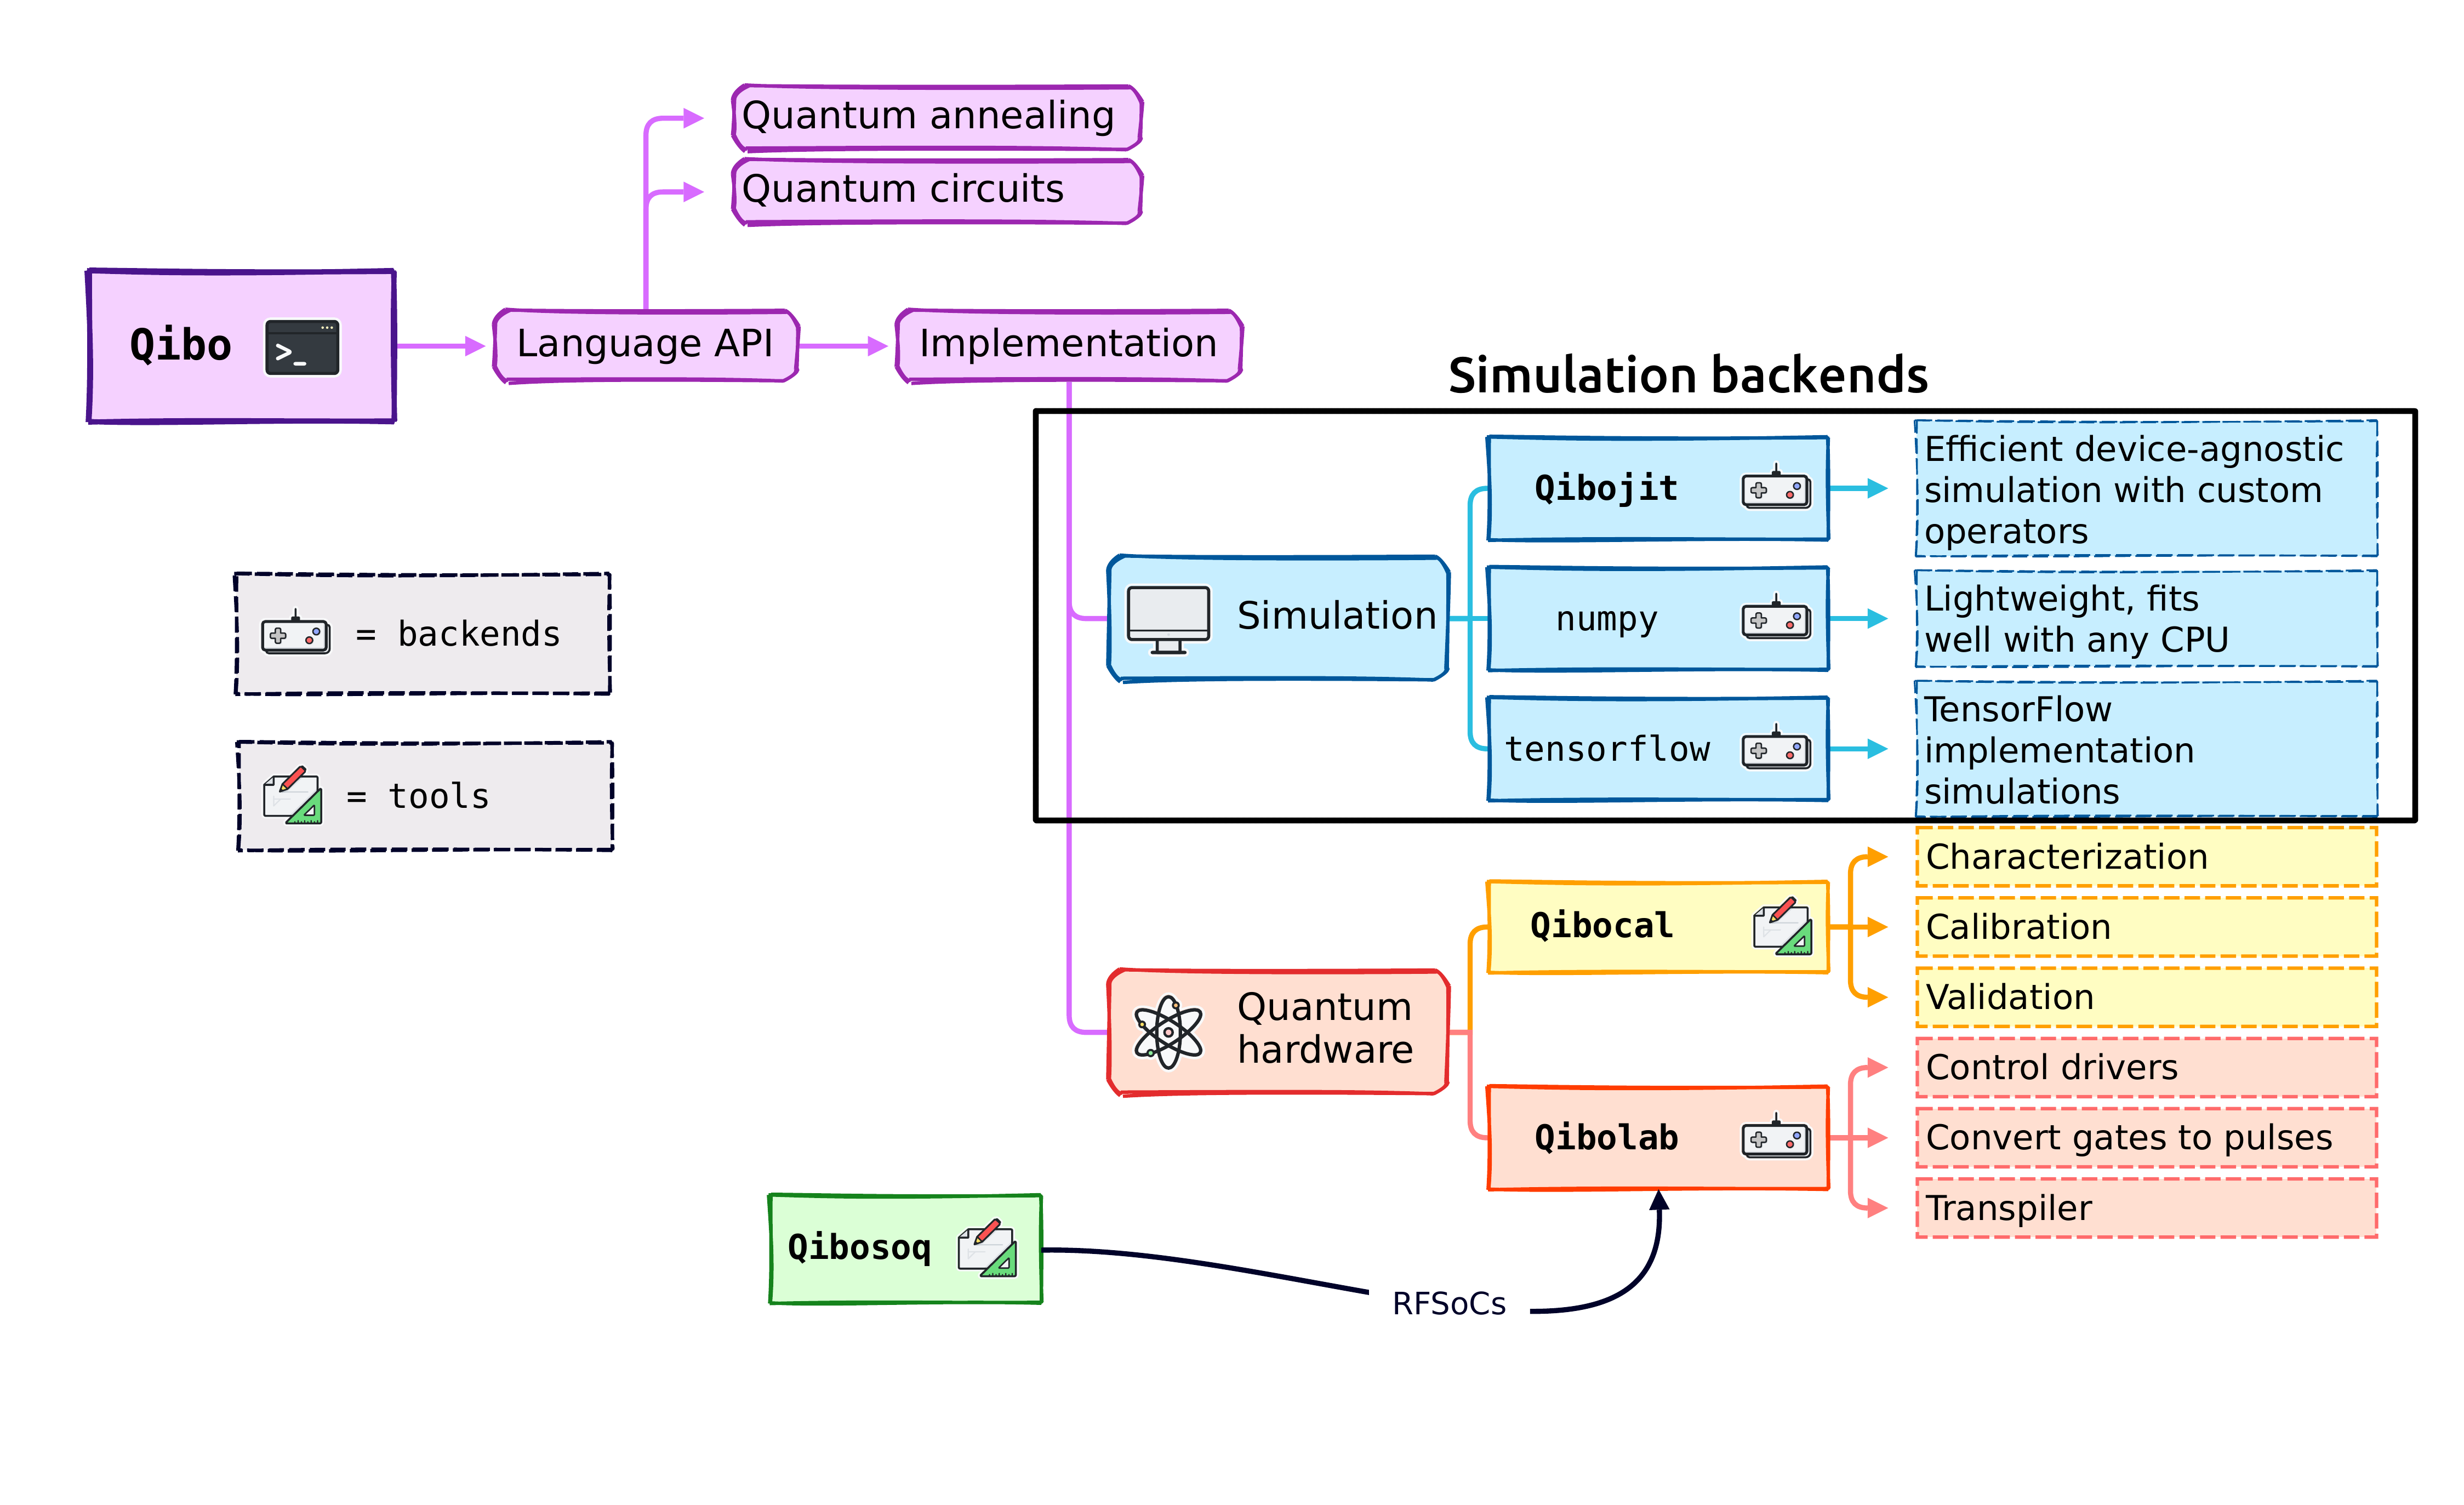
\includegraphics[width=1\textwidth]{figures/eco2.png}
\end{figure}
\end{frame}

\begin{frame}{My playground: \texttt{Qibo}}
\begin{figure}  
   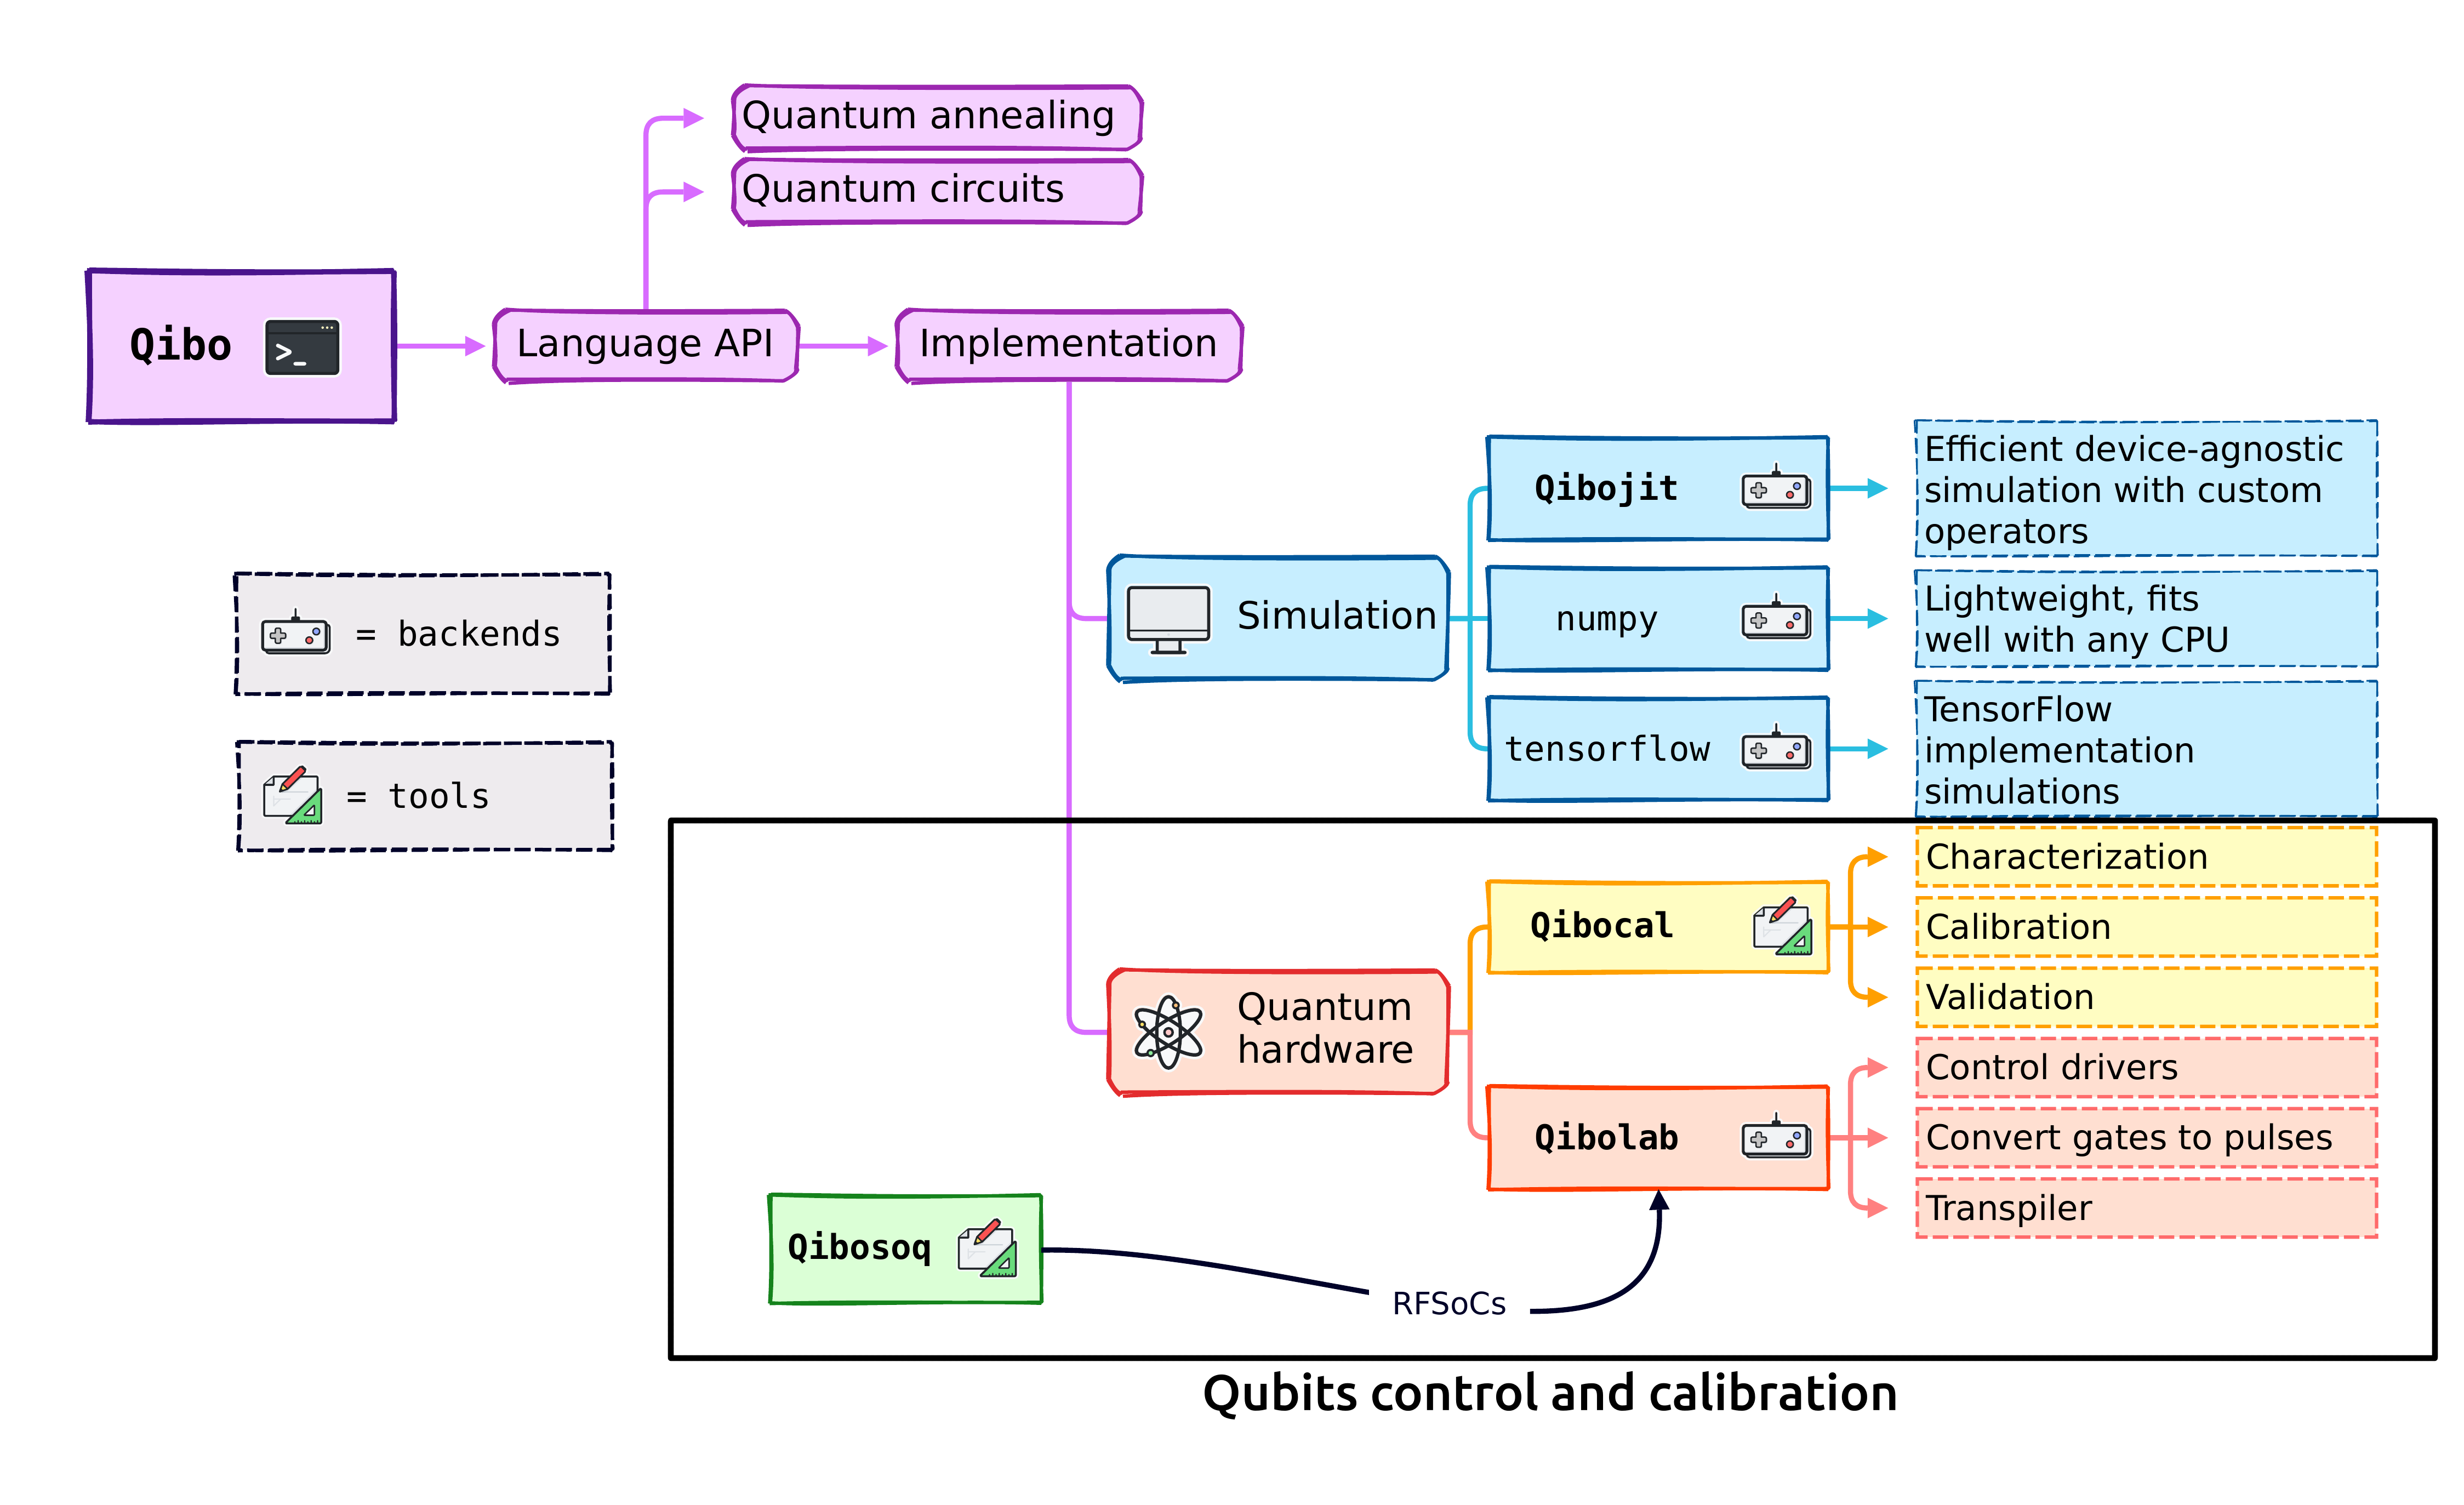
\includegraphics[width=1\textwidth]{figures/eco3.png}
\end{figure}
\end{frame}

\section{A target from HEP}

\begin{frame}{Parton Distribution Functions as QML target}
Taking one parton $p_i$, we can see its PDF as the probability for $p_i$ of carring 
a fraction $x$ of the momentum of the proton.
\begin{figure}  
   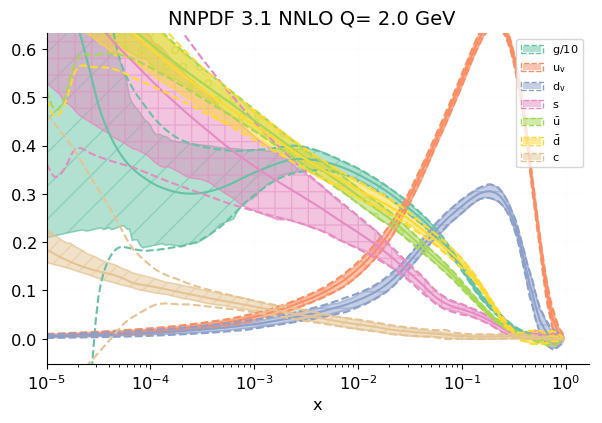
\includegraphics[width=0.75\textwidth]{figures/pdf.png}
\end{figure}
\end{frame}


\begin{frame}{The first (algorithmic) step \hfill \href{https://arxiv.org/abs/2011.13934}{\faBook\,\,arXiv:2011.13934}}
\pause
\begin{multicols}{2}
$\,$
\begin{itemize}[noitemsep]
  \item[\footnotesize\faCircle] Define a circuit $\mathcal{U}(\bm{x};\bm{\theta})$ using one qubit per parton $p_i$;
  \item[\footnotesize\faCircle] fill gates with both $x_i$ and $\log(x_i)$;
  \item[\footnotesize\faCircle] Compute $\text{PDF}_i$ prediction using expectation of $Z_i = \bigotimes_{j=0}^n Z^{\delta_{ij}}:$
\end{itemize}
$$ \text{qPDF}_i(x_i; Q_0, \bm{\theta}) = \frac{1 - \braket{0|\mathcal{U}^{\dagger} Z_i \,
\mathcal{U}| 0}}{1 + \braket{0|\mathcal{U}^{\dagger} Z_i\, \mathcal{U}| 0}}  $$
\begin{figure}  
  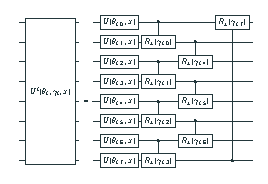
\includegraphics[width=0.5\textwidth]{figures/qpdf_circuit.pdf}
\end{figure}
\end{multicols}
\pause
\begin{figure}  
  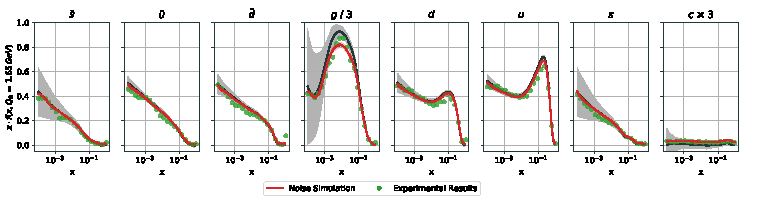
\includegraphics[width=1\textwidth]{figures/qpdf.pdf}
\end{figure}
\end{frame}

\begin{frame}{What if we run on hardware? \hfill \href{https://arxiv.org/abs/2308.06313}{\faBook\,\,arXiv:2308.06313}}
\pause
\begin{itemize}[noitemsep]
\item[\faCrosshairs] We take into account the $u$-quark PDF;
\pause
\item[\faExpand] we pre-process it to fit the range $[0,1]$;
\pause
\item[\faGamepad] we use \texttt{Qibo}, \texttt{Qibolab} and \texttt{Qibocal} to run a gradient descent.
\end{itemize}
\pause
\begin{figure}  
  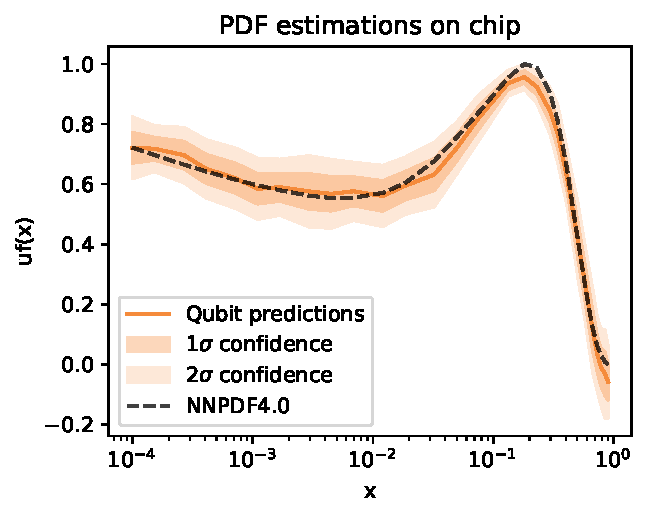
\includegraphics[width=0.5\textwidth]{figures/qpdf_full_stack.pdf}%
  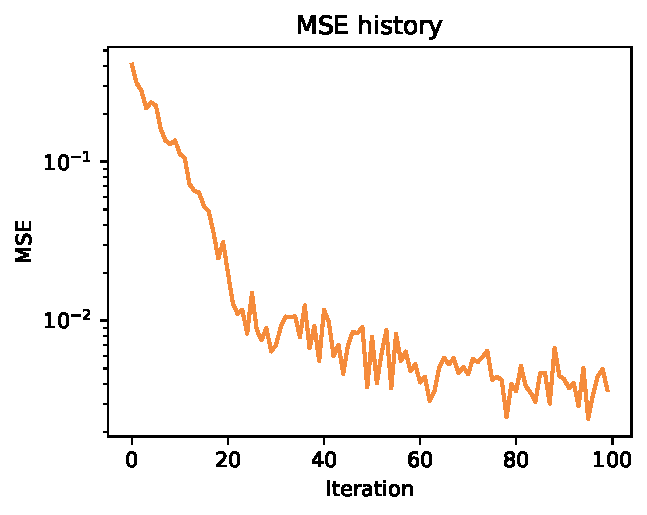
\includegraphics[width=0.5\textwidth]{figures/loss.pdf}%
\end{figure}
\pause
\begin{table}[ht]
\centering
\begin{tabular}{ccccccccc}
\hline \hline 
\rule{0pt}{2.5ex}
\textbf{Parameter} & $N_{\rm train}$ & $N_{\rm params}$ & Optimizer & $N_{\rm shots}$ & $\text{MSE}_{\rm final}$ & $T_{\rm exe}$ \\
\hline
\rule{0pt}{2.5ex}
\textbf{Value} & $30$ & $14$ & Adam & $250$ & $3.6\cdot 10^{-3}$ & $78'$ \\
\hline \hline 
\end{tabular}
\label{tab:qml}
\end{table}
\end{frame}

\begin{frame}{What if we run on hardware?\hfill \href{https://arxiv.org/abs/2308.06313}{\faBook\,\,arXiv:2308.06313}}
\begin{itemize}[noitemsep]
\item[\faCrosshairs] We take into account the $u$-quark PDF;
\item[\faExpand] we pre-process it to fit the range $[0,1]$;
\item[\faGamepad] we use \texttt{Qibo}, \texttt{Qibolab} and \texttt{Qibocal} to run a gradient descent.
\end{itemize}
\begin{figure}  
  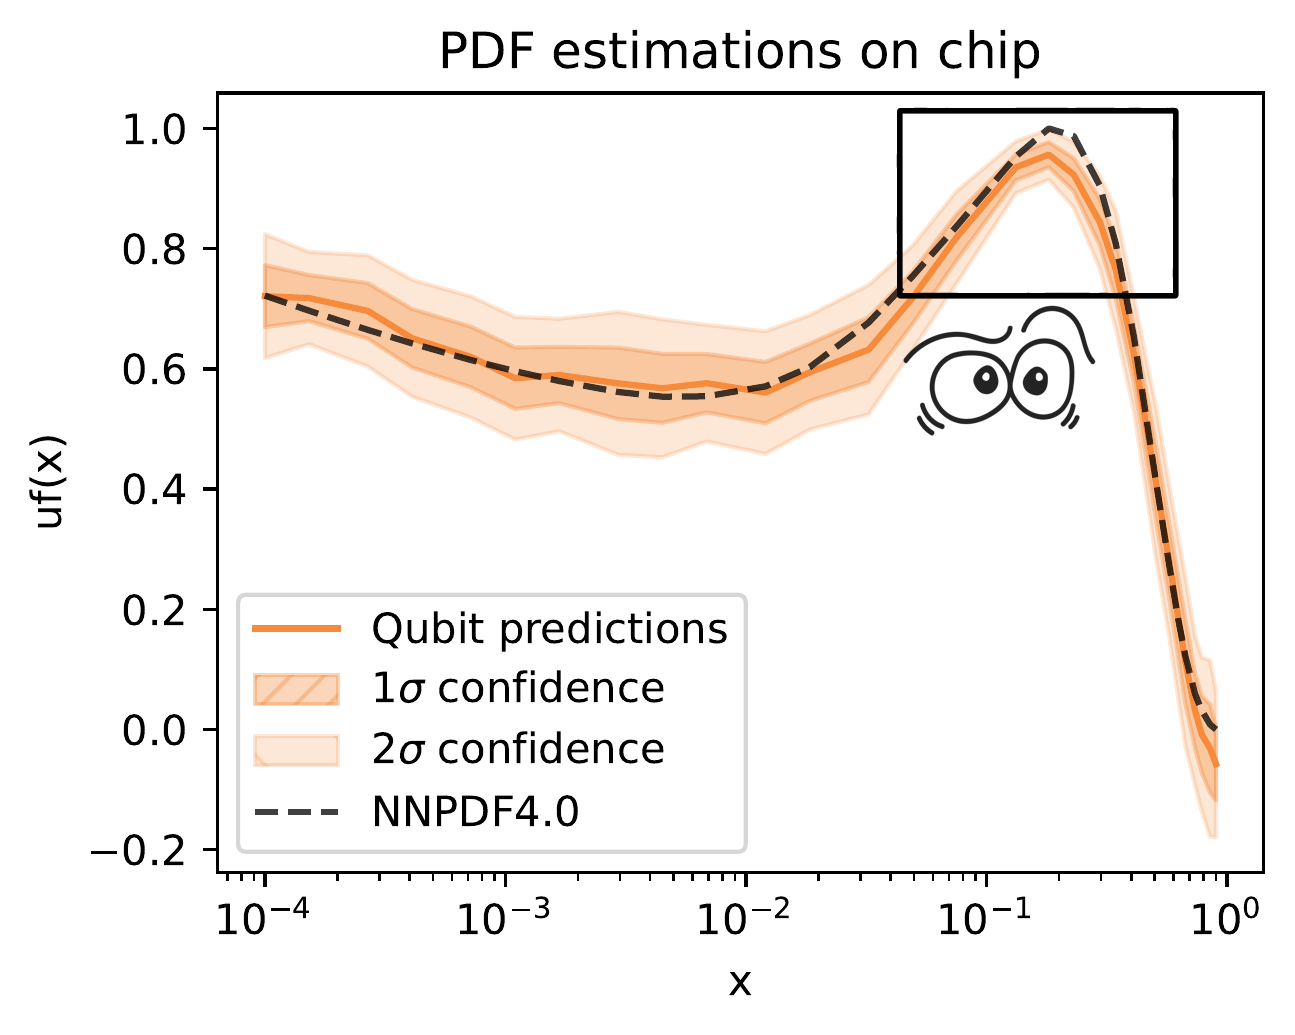
\includegraphics[width=0.5\textwidth]{figures/emo.png}%
  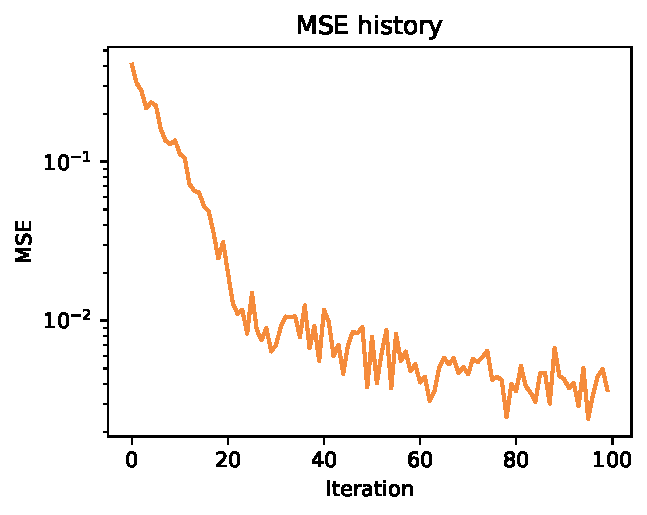
\includegraphics[width=0.5\textwidth]{figures/loss.pdf}%
\end{figure}
\begin{table}[ht]
\centering
\begin{tabular}{ccccccccc}
\hline \hline 
\rule{0pt}{2.5ex}
\textbf{Parameter} & $N_{\rm train}$ & $N_{\rm params}$ & Optimizer & $N_{\rm shots}$ & $\text{MSE}_{\rm final}$ & $T_{\rm exe}$ \\
\hline
\rule{0pt}{2.5ex}
\textbf{Value} & $30$ & $14$ & Adam & $250$ & $3.6\cdot 10^{-3}$ & $78'$ \\
\hline \hline 
\end{tabular}
\label{tab:qml}
\end{table}
\end{frame}

\begin{frame}{Quantum error mitigation\hfill \href{https://arxiv.org/abs/2005.10189}{\faBook\,\,arXiv:2005.10189}}
\faLightbulbO\,\, Idea: learning a noise map $\ell$ and use it to clean expectation values from noise:
$$ \braket{\mathcal{O}}_{\rm clean} = \ell\bigl[ \braket{\mathcal{O}}_{\rm noisy} \bigr] $$
\pause 
\begin{figure}
    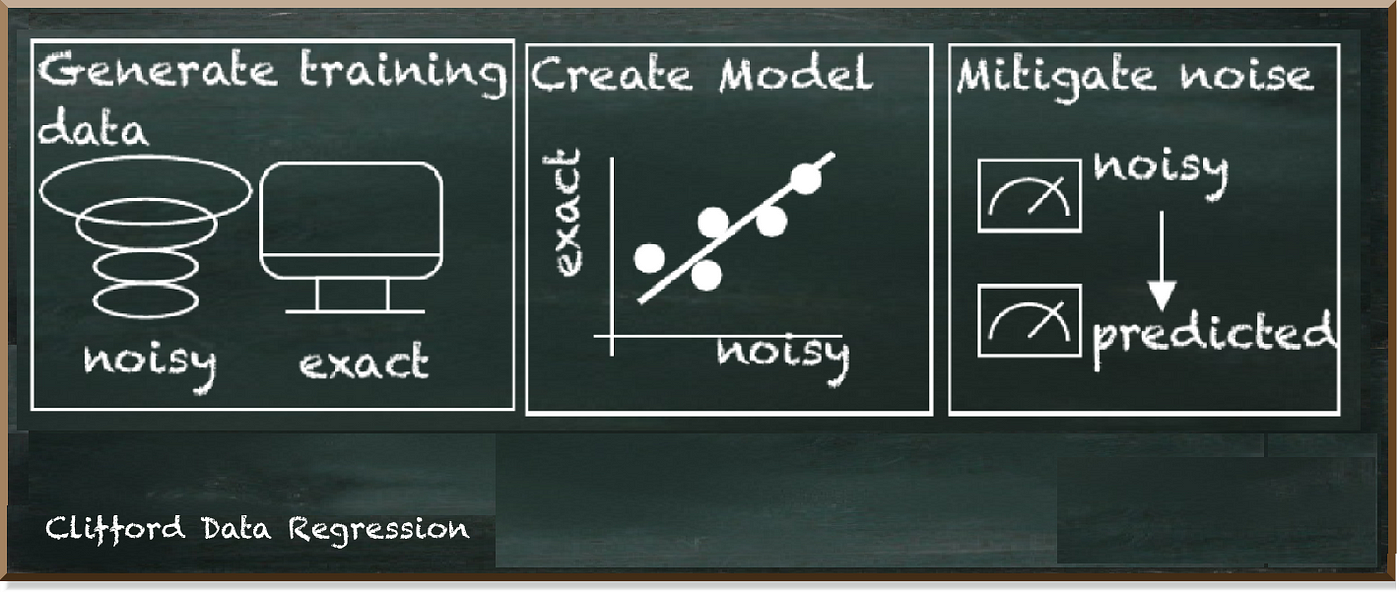
\includegraphics[width=1\textwidth]{figures/cdr.png}
    \caption*{Credits: Frank Zickert.}
\end{figure}
\end{frame}

\begin{frame}{Real time quantum error mitigation\hfill \href{https://arxiv.org/abs/2311.05680}{\faBook\,\,arXiv:2311.05680}}
\pause
We try to mitigate both gradients and predictions at each optimization iteration.
\pause
\begin{figure}
    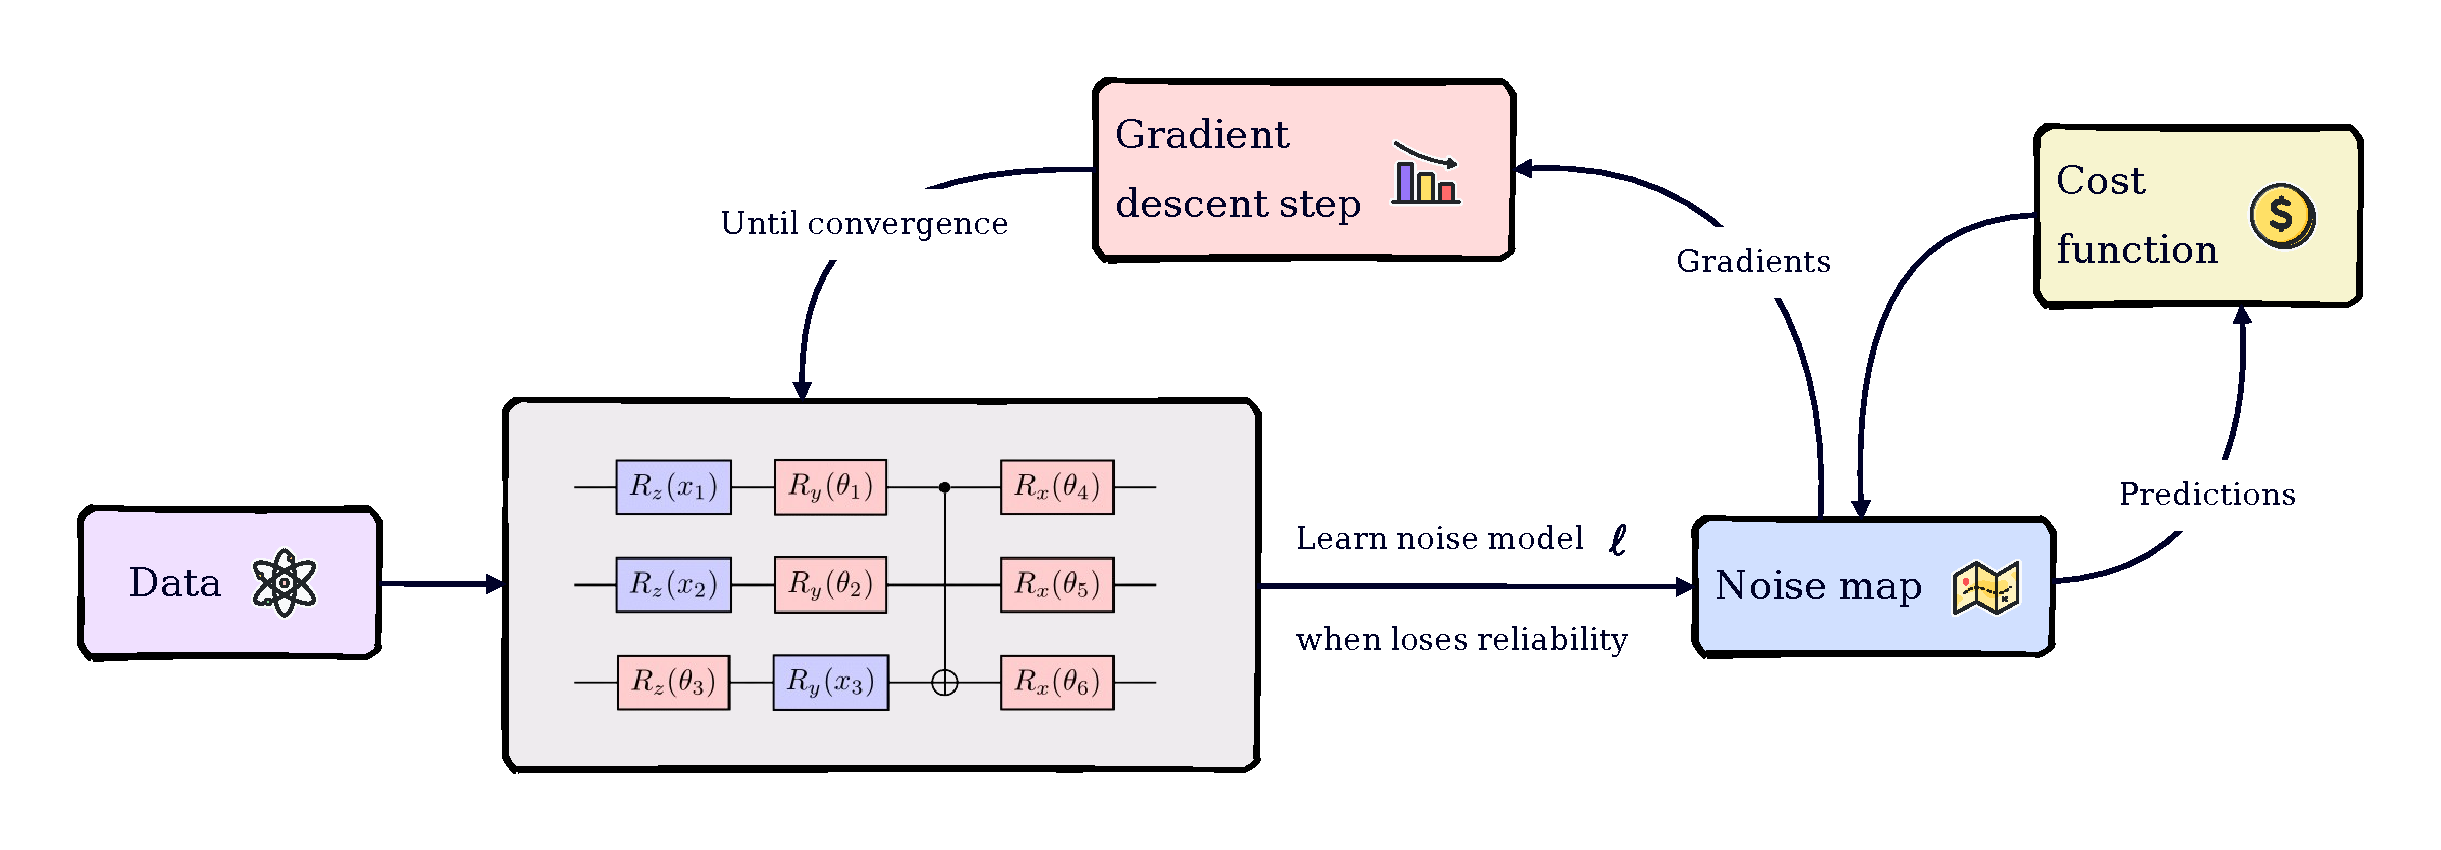
\includegraphics[width=1\textwidth]{figures/rtqem.pdf}
\end{figure}
\pause
\begin{itemize}[noitemsep]
\item[\faClockO] these experiments take long execution times (but we have \texttt{Qibo}!);
\pause
\item[\faLeaf] in some regimes, we aim to remove the bounds imposed by noise.
\end{itemize}
\end{frame}

\begin{frame}{RTQEM in action\hfill \href{https://arxiv.org/abs/2311.05680}{\faBook\,\,arXiv:2311.05680}}
\begin{center}
\footnotesize
\begin{tabular}{ccccccccc}
\hline \hline 
\rule{0pt}{2.5ex}
\textbf{Parameter} & $N_{\rm train}$ & $N_{\rm params}$ & $N_{\rm shots}$ 
& $\text{MSE}_{\rm rtqem}$ &  $\text{MSE}_{\rm nomit}$ & Noise \\
\hline
\rule{0pt}{2.5ex}
\textbf{Value} & $30$ & $16$ & $10^{4}$ &  $0.008$ & $0.018$ & local Pauli \\
\hline \hline 
\end{tabular}
\end{center}

\begin{figure}
    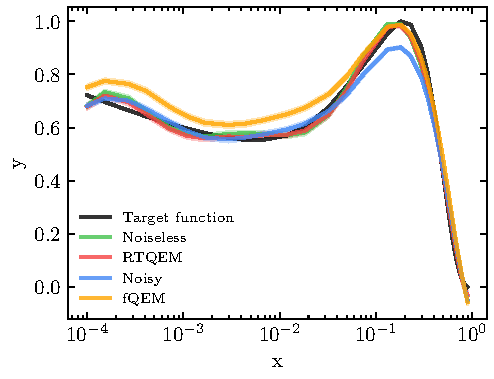
\includegraphics[width=0.485\textwidth]{figures/qpdf_sim.pdf}%
    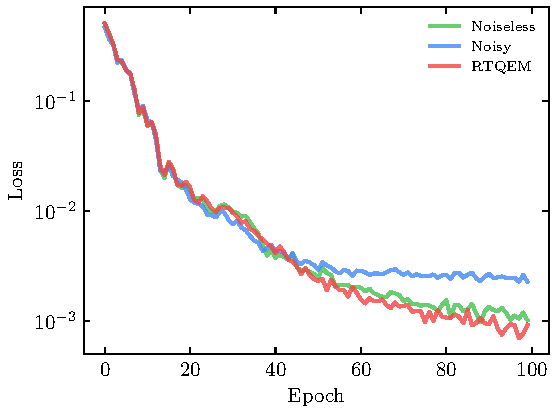
\includegraphics[width=0.5\textwidth]{figures/qpdf_loss.pdf}
\end{figure}
\begin{itemize}[noitemsep]
\item[1.] thanks to the RTQEM procedure, we reach a good minimum of the cost function;
\item[2.] the QEM is not effective if applied to a corrupted scenario (orange curve).
\end{itemize}
\end{frame}

\begin{frame}{RTQEM on a superconducting qubit\hfill \href{https://arxiv.org/abs/2311.05680}{\faBook\,\,arXiv:2311.05680}}
\begin{center}
\footnotesize
\begin{tabular}{ccccccccc}
\hline \hline 
\rule{0pt}{2.5ex}
\textbf{Parameter} & $N_{\rm train}$ & $N_{\rm params}$ & $N_{\rm shots}$ & $\text{MSE}_{\rm rtqem}$ &  $\text{MSE}_{\rm nomit}$ 
& Noise \\
\hline
\rule{0pt}{2.5ex}
\textbf{Value} & $15$ & $16$ & $500$ & $0.0042$ & $0.0055$ & real noise\\
\hline \hline 
\end{tabular}
\end{center}

\begin{figure}
    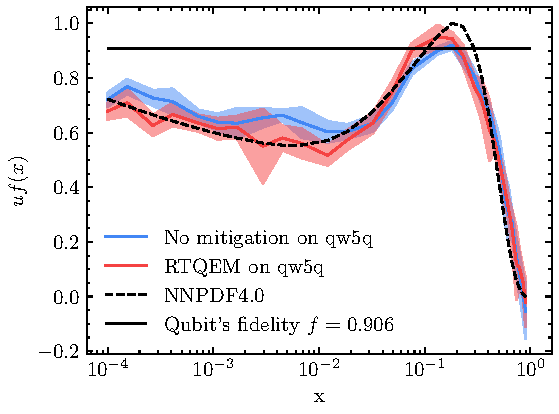
\includegraphics[width=0.5\textwidth]{figures/qw5q_short.pdf}%
    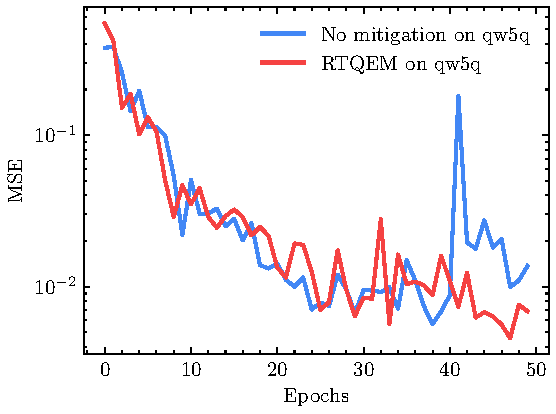
\includegraphics[width=0.5\textwidth]{figures/losses_qw5q.pdf}
\end{figure}
\vspace{0.4cm}
\centering
RTQEM allows exceeding the natural bound imposed by noise.
\end{frame}

\begin{frame}{Can RTQEM generalise?\hfill \href{https://arxiv.org/abs/2311.05680}{\faBook\,\,arXiv:2311.05680}}
We perform a longer training on two different devices (and noises!) using the same 
initial conditions of the previous slide but $N_{\rm epochs}=100$. 
\pause
\begin{multicols}{2}

\begin{figure}
    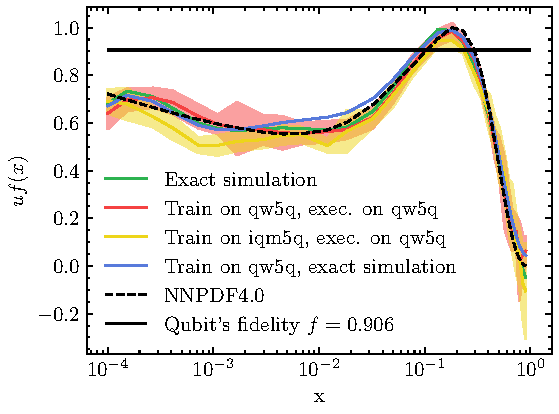
\includegraphics[width=0.5\textwidth]{figures/100.pdf}%
\end{figure}
\pause
\begin{center}
\begin{itemize}[noitemsep]
  \item[\faCog] \textbf{\texttt{qw5q}} from QuantWare and controlled using Qblox instruments;
  \item[\faCog] \textbf{\texttt{iqm5q}} from IQM and controlled using Zurich Instruments.
\end{itemize}
\pause
\footnotesize
\begin{table}
\begin{tabular}{ccccc}
\hline \hline 
\textbf{Train.} & \textbf{Epochs} & \textbf{Pred.} &  \textbf{Config.} & MSE \\
\hline    
\texttt{qw5q} & 50 & \texttt{qw5q} & noisy & $0.0055$  \\     
\texttt{qw5q} & 50 & \texttt{qw5q} & RTQEM & $0.0042$ \\ 
\hline 
\texttt{qw5q} & 100 & \texttt{qw5q} & RTQEM & $0.0013$  \\     
\texttt{iqm5q} & 100 & \texttt{qw5q} & RTQEM & $0.0037$ \\   
\texttt{qw5q} & 100& \texttt{sim} & RTQEM & $0.0016$ \\   
\hline \hline
\end{tabular}
\centering
\end{table}
\end{center}
\end{multicols}
\pause
All the hardware results are obtained deploying the $\bm{\theta}_{\rm best}$ on 
\texttt{qw5q}.
\end{frame}

\begin{frame}
\begin{figure}
    
\includegraphics[width=1\textwidth]{figures/thank.png}%
\end{figure}
\end{frame}

\end{document}
